\documentclass[11pt,oneside]{book}

% per stampare fronteretro
%\documentclass[11pt,twoside]{book}

%\captionheaderfont{\sl\bfseries}
%\captionbodyfont{\sl}

%%\renewcommand{\tableshortname}{Table}
%%\renewcommand{\figureshortname{Figure}
%%\chapapp{\chaptername}
\usepackage[italian,english]{babel}
\usepackage[utf8]{inputenc}
\usepackage[T1]{fontenc}

\usepackage{epsfig}
\usepackage{psfig}
\usepackage{subfig}
\usepackage{cite}
\usepackage{amsmath}
\usepackage{latexsym}
%\usepackage[italian]{minitoc}
\usepackage{fancybox}

\usepackage{psfig}
\usepackage{verbatim}
\usepackage{url}
\usepackage{graphicx}
\usepackage{color}
%\usepackage{concmath}
\usepackage{moreverb}

\usepackage{tikz}
\usetikzlibrary{arrows}

%HYPERREF per uso con dvi
%\usepackage[final,backref,breaklinks,pagebackref,colorlinks]{hyperref}
%HYPERREF per uso con con pdf (con bookmark)
%\usepackage[final,bookmarks,backref,breaklinks,dvips,colorlinks]{hyperref}\\
\usepackage[final,bookmarks,backref,breaklinks,colorlinks]{hyperref}
%mypackages
\usepackage{listings}

\newlength{\realtextwidth}

%%%%% marginpar macros and new realtextwidth
\newcommand{\margintext}[1]
{\mbox{}\marginpar{\sf\tiny\bf\hspace{0pt}#1}}
\marginparwidth 60pt
\setlength{\realtextwidth}{380pt}
%\setlength{\realtextwidth}{\textwidth}
%\addtolength{\realtextwidth}{\marginparwidth}
%\addtolength{\realtextwidth}{\marginparsep}




%%%%%%%%%%%%%%%%%%%%%%%%
%--------------------------------------------------
% MACROs
%--------------------------------------------------
\newcommand{\commento}[1]{\begin{quote}{\small\it #1}\end{quote}}
\newenvironment{javacode}{\begin{changemargin}{30pt}{0pt}\ \nopagebreak[4]\newline\noindent\small
%\smallskip\hrulefill\newline\noindent%linea da eliminare 
}
{\noindent\nopagebreak[4]\normalsize
\end{changemargin}\noindent
%\hrulefill\smallskip%linea  da eliminare
}
\newcommand{\codice}[1]{{\tt #1}}


\newcommand{\nota}[1]{\begin{center}\fbox{{\footnotesize\tt #1}}\end{center}}


\newenvironment{boxedpar}{\begin{center}
\begin{tabular}{|p{\figtextwidth}|} \hline}{\\ \hline
\end{tabular}\end{center}}

%per la visualizzazione di interazioni a video (compilazioni etc.)
\newenvironment{monitor}{\begin{boxedpar}\begin{verbatim}}
{\end{verbatim}\end{boxedpar}}


% Environment changemargine: Esempio: \begin{changemargin}{0pt}{-60pt}
\newenvironment{changemargin}[2]{%
 \begin{list}{}{%
  \setlength{\topsep}{0pt}%
  \setlength{\leftmargin}{#1}%
  \setlength{\rightmargin}{#2}%
  \setlength{\listparindent}{\parindent}%
  \setlength{\itemindent}{\parindent}%
  \setlength{\parsep}{\parskip}%
 }%
\item[]}{\end{list}}

\newcommand{\rosso}{\centerline{\color[rgb]{1.00,0.00,0.00}\fbox{Rosso}}}
\newcommand{\verde}{\centerline{\color[rgb]{0.00,1.00,0.00}\fbox{Verde}}}
%-------------------------------- end MACROs



%%%%% Larghezza e lunghezza massima delle figure
\newlength{\figtextwidth}
\setlength{\figtextwidth}{\textwidth}
\addtolength{\figtextwidth}{-12pt}
\newlength{\smallfigtextwidth}
\setlength{\smallfigtextwidth}{\textwidth}
\addtolength{\smallfigtextwidth}{-70pt}
\newlength{\figmaxheight}
\setlength{\figmaxheight}{\textheight}
\addtolength{\figmaxheight}{-2truecm}

% per il package verbatimtab:la dimensione del tab
\renewcommand\verbatimtabsize{4\relax}





\begin{document}
\selectlanguage{italian}

\begin{titlepage}
\begin{center}
\begin{center}

\includegraphics[scale=0.28, natwidth=793, natheight=1123]{img/logounisa.jpg}
\end{center}
{\Large Universit\`a degli Studi di Salerno}\\[0.2truecm]
{\large Facolt\`a di Scienze Matematiche Fisiche e Naturali}\\
\hrulefill
\vfill
{\large Tesi di Laurea Magistrale in}\\[0.2truecm]
{\Large Informatica}\\
\vfill\vfill
{\Huge Titolo}
\vfill\vfill


\ \ \ \ \ \ \ {\bf Relatori} \hfill {\bf Candidato}\ \ \\
Prof. Vincenzo Auletta \hfill Francesco Farina\\
Dott. Diodato Ferraioli \hfill Matricola 0522500282

\vfill
\hrulefill 

Anno Accademico 2015-2016

\end{center}
\end{titlepage}

\pagenumbering{roman}

\chapter*{Dediche e ringraziamenti}
\vfill


\vfill

{\hypersetup{linkcolor=black}
	\tableofcontents
}

%%%%%%%%%%%%%%%%%%%%%%%%%%%%
\chapter{Introduzione}
\setcounter{page}{1} 		% devono seguire solo il primo capitolo
\pagenumbering{arabic}	% devono seguire solo il primo capitolo
%%%


%%%%%%%%%%%%%%%%%%%%%%%%%%%%
\chapter{Alcuni concetti base}
\section{Teoria dei Grafi}
La teoria dei grafi è una branca della matematica, nata nel 1700 con Eulero, che consente di descrivere le relazioni che intercorrono tra un insieme di oggetti. Il grafo è lo strumento attraverso il quale tali relazioni possono essere espresse ed organizzate. Infatti, il grafo, consiste di oggetti chiamati \textit{nodi} e relazioni tra coppie di questi oggetti detti \textit{archi}; nodi connessi tra loro da un arco sono detti \textit{vicini} o \textit{adiacenti}.\\
\begin{figure}[h!]
	\centering
	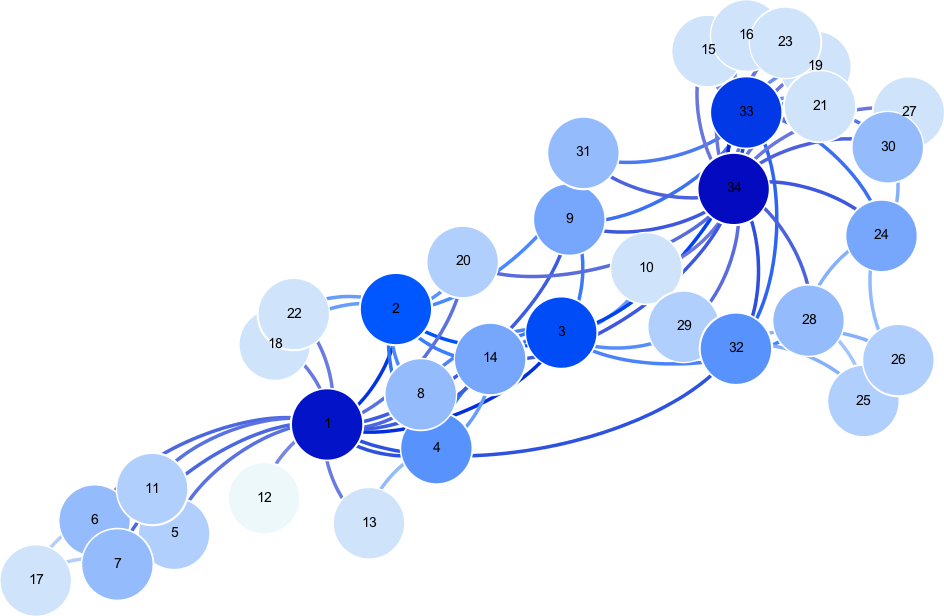
\includegraphics[scale=.3]{img/zkc.png}
	\caption{Grafo dello Zachary Karate Club.}
\end{figure}
\newpage
La relazione tra una coppia di nodi può essere di due tipi:
\begin{itemize}
	\item Simmetrica: l'arco connette i nodi con un collegamento bidirezionale ed è detto \textit{indiretto}. Un grafo costituito di soli archi indiretti è anch'esso detto indiretto.
	\item Asimmetrica: l'arco connette i nodi con un collegamento unidirezionale ed è detto \textit{diretto}. Un grafo costituito di soli archi diretti è anch'esso detto diretto.
\end{itemize}
\begin{figure}[h!]
	\vspace*{1cm}
	\begin{minipage}{0.45\textwidth}
	\centering
	\begin{tikzpicture}[-,>=stealth',shorten >=1pt,auto,node distance=2cm,
		thick,main node/.style={circle,draw,font=\sffamily\Large\bfseries}]
		\node[main node] (1) {1};
		\node[main node] (2) [below left of=1] {2};
		\node[main node] (3) [below right of=2] {3};
		\node[main node] (4) [below right of=1] {4};
		\path[every node/.style={font=\sffamily\small}]
		(1) edge node [left] {} (4)
		
		(2) edge node [right] {} (1)
		
		(3) edge node [right] {} (2)
		
		(4) edge node [left] {} (3);
		
	\end{tikzpicture}
	\caption{Grafo indiretto}
	\end{minipage}\hfill
% <-- needed to keep the imgs side by side
	\begin{minipage}{0.45\textwidth}
	\centering
	\begin{tikzpicture}[->,>=stealth',shorten >=1pt,auto,node distance=2cm,
		thick,main node/.style={circle,draw,font=\sffamily\Large\bfseries}]
		\node[main node] (1) {1};
		\node[main node] (2) [below left of=1] {2};
		\node[main node] (3) [below right of=2] {3};
		\node[main node] (4) [below right of=1] {4};
		\path[every node/.style={font=\sffamily\small}]
		(1) edge node [left] {} (4)
		
		(2) edge node [right] {} (1)
		
		(3) edge node [right] {} (2)
		
		(4) edge node [left] {} (3);
	\end{tikzpicture}
	\caption{Grafo diretto}
	\end{minipage}
\end{figure}
Un grafo può essere formalmente descritto come una coppia di insiemi \textbf{G = (V, E)}, dove V è l'insieme dei nodi ed E è l'insieme degli archi. Un arco e $\in$ E è rappresentato come un sottoinsieme di due elementi di V, $e = \lbrace u, v\rbrace$ per $u, v \in V$.\\
Le rappresentazioni atte a descrivere un grafo sono molteplici:
\begin{itemize}
	\item \textit{Rappresentazione grafica}: ad ogni nodo corrisponde una figura circolare sul piano e ad ogni arco (i, j) corrisponde una linea che che collega il nodo i al nodo j.
	\item \textit{Matrice di adiacenza}: matrice di dimensione $n \times n$, dove $n$ è il numero di nodi, il cui elemento (i, j) assume valore 1 se esiste l'arco tra il nodo i ed il nodo j, 0 altrimenti.
	\item \textit{Lista di adiacenza}: ad ogni vertice $v$ è associata la lista dei nodi ad esso vicini.
\end{itemize}
Negli anni, gli studi sulla teoria dei grafi hanno prodotto una quantità enorme di definizioni e teoremi, per cui, di seguito vengono descritti solamente i concetti necessari alla comprensione di questo lavoro di tesi.
\paragraph{Sottografo.} Un grafo H si dice sottografo di un grafo G se i vertici di H sono un sottoinsieme dei vertici di G e gli archi di H sono un sottoinsieme degli archi di G. Siano $G=(V, E)$ ed $H=(V_1, E_1)$ due grafi. H è un sottografo di G se e solo se $V_1 \subseteq V$ ed $E_1 \subseteq E$.
Un concetto particolarmente utile alla comprensione di questo lavoro è lo \textit{spanning subgraph}: uno spanning subgraph H di un grafo G è un sottografo che contiene tutti i vertici di G, cioé $V_1 = V$.
\paragraph{Grado di un nodo.} Il grado di un nodo $v$ è il numero di nodi ad esso adiacenti ed è indicato con \textit{deg(v)}.\\
In un grafo diretto, si distinguono due tipi di grado:
\begin{itemize}
	\item \textit{in-deg(v)}, il grado in ingresso del nodo \textit{v}, dato dal numero di archi in cui \textit{v} compare come nodo destinazione;
	\item \textit{out-deg(v)}, il grado in uscita del nodo \textit{v}, dato dal numero di archi in cui \textit{v} compare come nodo sorgente.
\end{itemize}
\paragraph{Cammino.} Un cammino è una sequenza di nodi, in cui ogni coppia consecutiva della sequenza sia connessa da un arco. Formalmente, un cammino è una sequenza di vertici $v_0, v_1, \cdots, v_n \in V$ tale che $\lbrace v_{i-1}, v_i\rbrace \in E, \forall 1\leq i \leq n$. Un cammino con almeno tre vertici distinti, i cui vertici di inizio e fine coincidono, è detto \textit{ciclo}.
\paragraph{Grafo connesso.} Un grafo è connesso se, per ogni coppia distinta di vertici (i, j), esiste un cammino da i a j.

\subsection{Reti Sociali}
Una rete sociale è un costrutto teorico proveniente dalle scienze sociali, utilizzata per studiare le relazioni fra individui, gruppi, organizzazioni ed intere società. Il termine rete sociale viene utilizzato per descrivere una struttura sociale determinata dalle interazione tra gli attori che la compongono\cite{scott}.
Tali reti sono quindi strutture relazionali tra attori ed in quanto tali costituiscono una forma sociale rilevante che definisce il contesto in cui si muovono quegli stessi attori. Una rete sociale risulta essere allora la struttura di relazioni, le cui caratteristiche potessero essere usate per spiegare, in tutto o in parte, il comportamento delle persone che la costituiscono. Elementi costitutivi della rete sociale sono dunque: 
\begin{itemize}
	\item I soggetti, che rappresentano le unità, i nodi che compongono la rete (individui, gruppi, posizioni, luoghi, etc.); 
	\item Le relazioni che legano i soggetti, che compongono la rete e che possiedono determinate caratteristiche.
\end{itemize}
Con riferimento al contenuto della relazione è possibile cogliere ed individuare alcune particolari reti che, per il tipo di legami che le costituiscono, si caratterizzano per essere reti di sostegno (supporto sociale):
\begin{itemize}
	\item \emph{Formali}, costituite dalle istituzioni sociali;
	\item \emph{Informali}, che non presentano una veste istituzionalmente definita;
	\item \emph{Primarie}, costituite da quelle relazioni, che in virtù dei legami naturali, accomunano gli individui, come rapporti familiari, parentali, di vicinato;
	\item \emph{Secondarie}, formate da relazioni di conoscenza indiretta;
	\item \emph{Complesse}, composte da un elevato numero di relazioni con caratteristiche specifiche.
\end{itemize}
Nell'ambito delle scienze sociali, il concetto di rete sociale è stato utilizzato a lungo come ``metafora'' per tradurre quelle che sono le idee di società e d'azione sociale, come esito di vincoli ed opportunità emergenti dalle relazioni tra i soggetti. L’uso metaforico del termine ha posto il concetto di rete sociale ad un livello di astrazione piuttosto elevato, creando confusione terminologica e mancanza di chiarezza. Successivamente, mediante l'impiego scientifico del termine, tale livello di astrazione è diminuito, determinando il passaggio del concetto di rete dall'immagine intuitiva di un fenomeno complesso alla sua rappresentazione sul piano formale ed analitico. Ciò ha portato le reti sociali, come rappresentazione organizzativa dei rapporti sociali ed il suo metodo di studio, \textbf{l’analisi delle reti sociali}, ad essere adottate come strumenti teorici e metodologici per lo studio di numerosi fenomeni e processi. In ambito sociologico, tali studi hanno mostrato che nelle reti si depositano valori materiali, ma soprattutto non materiali che contribuiscono a determinare la ``ricchezza'' individuale e collettiva (diversa da individuo ad individuo, non solo grazie alle capacità relazionali, ma anche per effetto di specifici processi strutturali)\cite{pisa}.
Quindi, \textit{l'analisi delle reti sociali} comprende principalmente tutta la parte teorica ed i modelli utilizzati per lo studio delle reti sociali in generale. Un esempio reale di una fitta rete sociale è quello mostrato in Figura \ref{fig:hp}. Di seguito, dopo alcuni cenni storici si passa alla descrizione di concetti e strumenti derivanti dalla \emph{teoria dei grafi} che è alla base della \textit{Social Network Analysis}.
\begin{figure}[ht]
	\centering \shadowbox{
		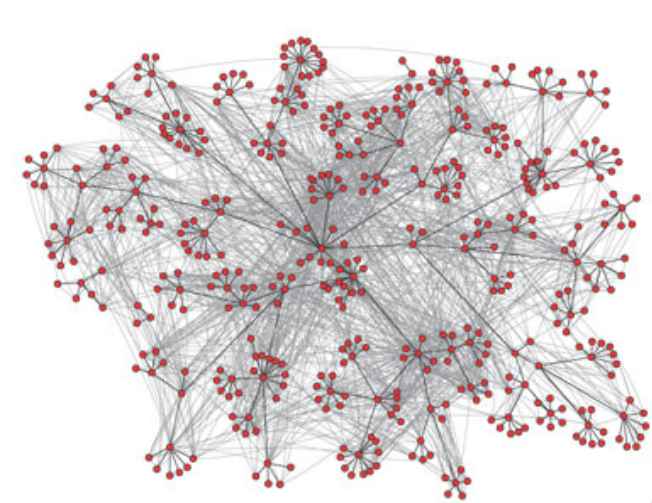
\includegraphics[scale=0.5]{img/hp.png}}
	\caption{Scambio di e-mail tra i 436 impiegati di HP Research Lab}
	\label{fig:hp}
\end{figure}

\subsection{Cenni storici}
L'idea delle reti sociali nacque verso la fine del 1900, grazie alle teorie e le ricerche su gruppi sociali di \textit{\`Emile Durkheim} e \textit{Ferdinand T\"{o}nnies}. Quest'ultimo sosteneva che i gruppi sociali possono esistere come legami personali e diretti, i quali collegano gli individui che condividono valori e credenze (\emph{community}), oppure impersonali e formali (\emph{società})\cite{tonnies}. Durkheim fornì una spiegazione non individualistica dei fenomeni sociali, affermando che essi sorgono quando gli individui interagiscono costituendo una realtà che non può più essere rappresentata, in termini di proprietà dei singoli\cite{durkheim}.
\\
Inoltre intorno al ventesimo secolo, \emph{Georg Simmel} si concentrò sulla natura delle reti e su quanto le dimensioni delle reti influenzassero le interazioni tra le componenti della rete, esaminandone le probabilità di interazione in reti debolmente collegate, piuttosto che in gruppi\cite{simmel}.
\\
Importanti sviluppi nel campo possono essere riscontrati intorno al 1930, grazie a differenti ed indipendenti gruppi di psicologi, antropologi e matematici. In psicologia, \emph{Jacob L. Moreno} iniziò una registrazione ed un'analisi sistematica delle interazioni sociali all'interno di piccoli gruppi. Per quanto riguarda l'antropologia, la fondazione della teoria delle reti sociali è dovuta ai lavori teorici ed entrografici di \emph{Bronislaw Malinowski}\cite{bronislaw}, \emph{Alfred Radcliffe-Brown}\cite{brown1, brown2}, e \emph{Claude Lévi-Strauss}\cite{strauss}, gruppo di antropologi sociali a cui vengono attribuiti i primi lavori di analisi di rete, investigando le community nel sud Africa, India e Regno Unito. In concomitanza a tale gruppo, l'antropologo inglese \emph{S.F. Nadel} codificò una teoria riguardante le strutture sociali che influenzò l'analisi delle reti\cite{nadel}. Nel campo della sociologia, nei primi anni del 1930 \emph{Talcott Parsons} preparò il terreno per l'adozione di un approccio relazionale per comprendere le struttura sociali \cite{parsons1, parsons2}. Successivamente, attingendo dalle teorie di Parsons, il lavoro del sociologo \emph{Peter Blau} sulla teoria dello scambio sociale fornì un forte impatto per l'analisi dei legami relazionali\cite{blau1,blau2,blau3}. A partire dal 1970, un numero crescente di studiosi lavorò per combinare le differenti tracce e tradizioni, fra cui un gruppo composto dal sociologo \emph{Harrison White} ed i suoi studenti del dipartimento di scienze sociale dell'università di Harvard. Ed in maniera indipendente, \emph{Charles Tilly} si concentrò sulle relazioni fra le dinamiche politiche e sociali, e \emph{Stanley Milgram} sviluppò la tesi sui sei gradi di separazione\cite{bernie}. In seguito, \emph{Mark Granovetter}\cite{grano} e \emph{Barry Wellman}\cite{wellman} furono fra i primi studenti di White ad elaborare e sostenere l'analisi delle reti sociali\cite{mullins, tillyc, wellman2}.

\subsection{Grafo come modello della realtà}
I grafi hanno una grande utilità, in quanto consentono di astrarre le relazioni che intercorrono tra più oggetti, e di rappresentare tali relazioni in strutture su cui è possibile applicare modelli matematici. In \cite{easley2010networks} viene proposto un esempio reale: la Figura \ref{arpanet} rappresenta la struttura della rete Internet nel Dicembre del 1970, noto come ARPANET allora, composto solo da 13 macchine. I nodi rappresentano gli host, e vi è un arco tra due host se esiste una comunicazione diretta tra di essi.
\begin{figure}[h!]
	\centering
	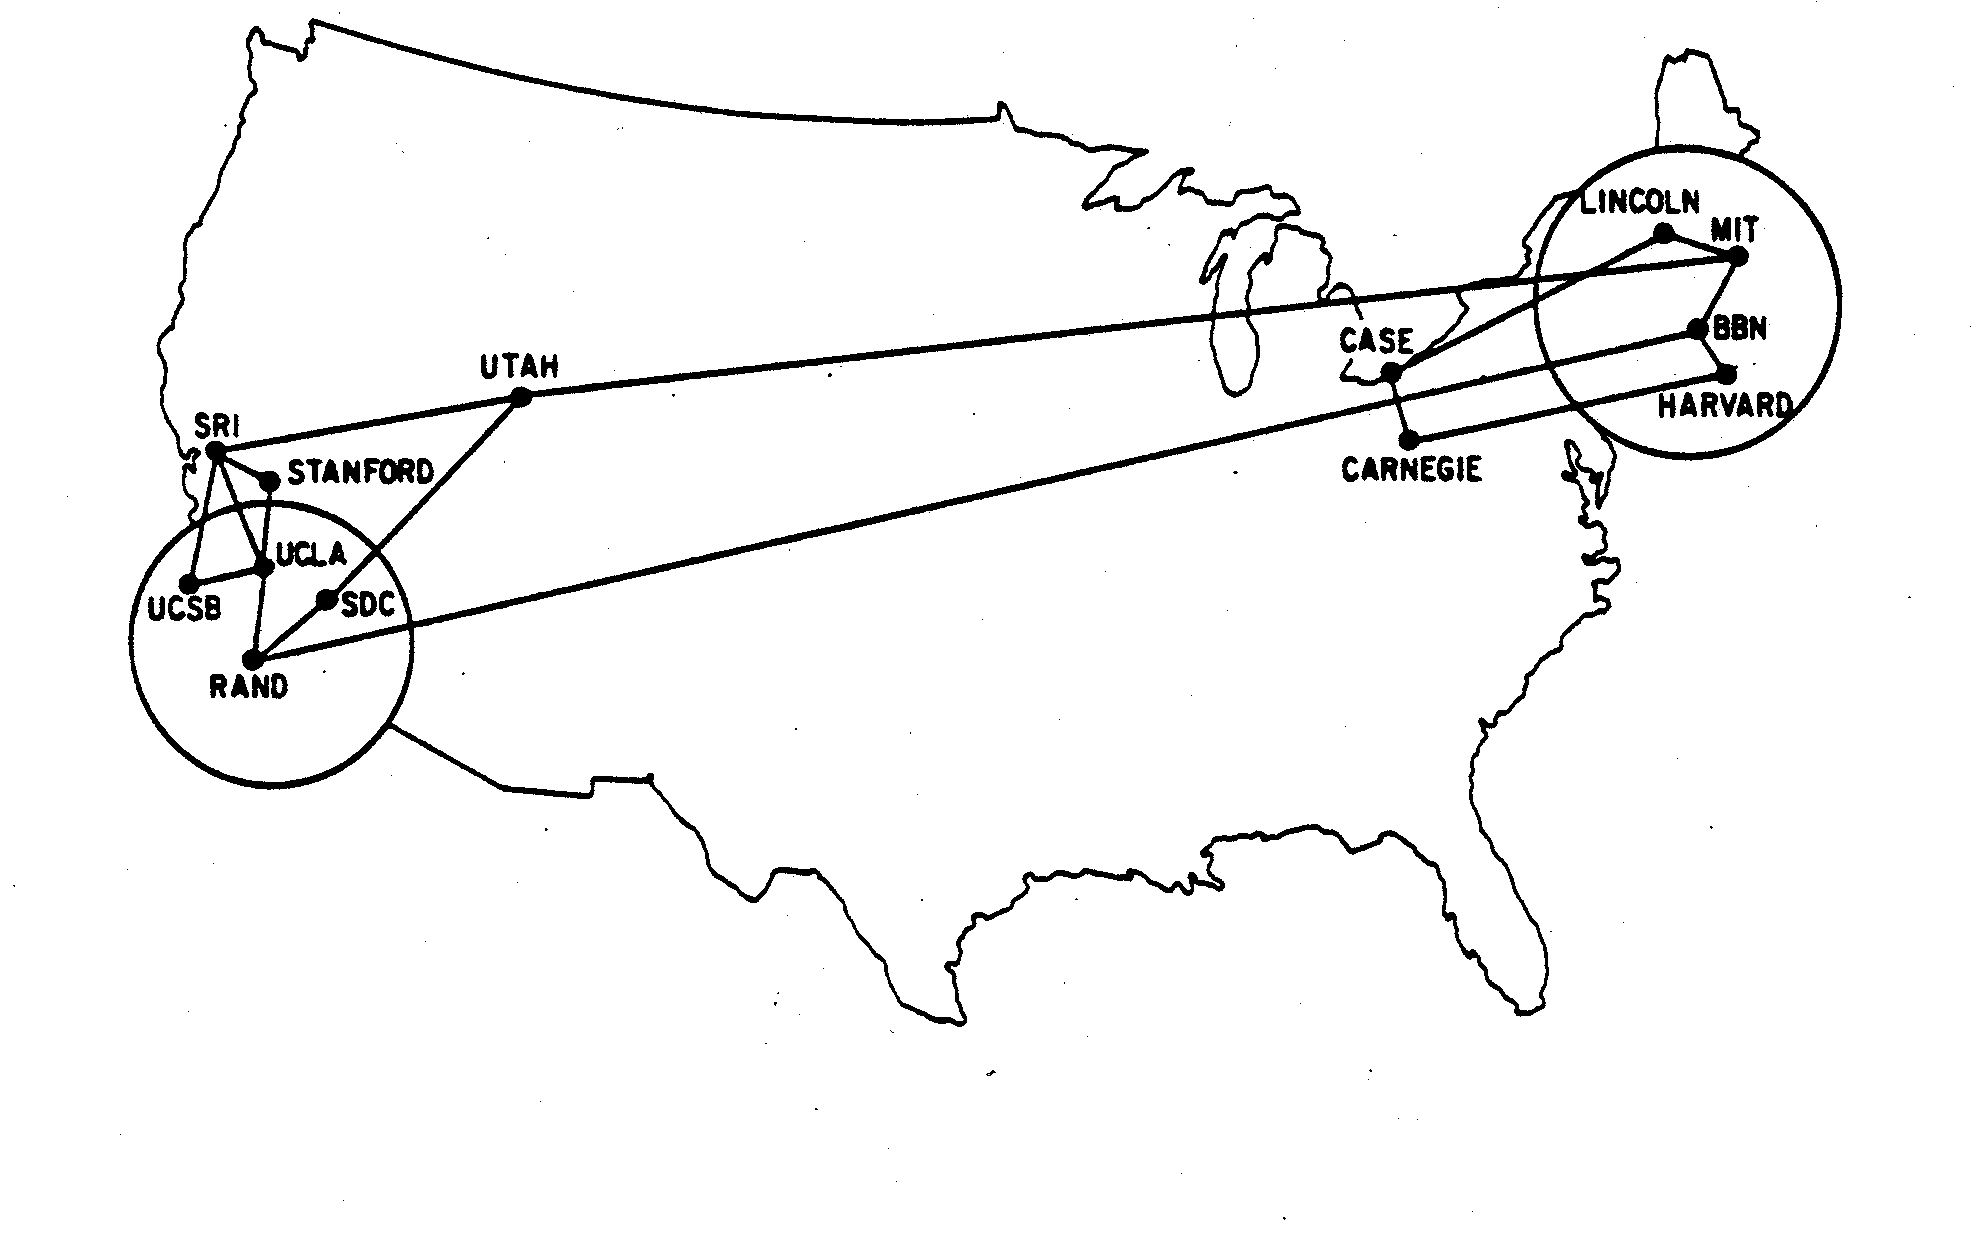
\includegraphics[scale=.7]{img/arpanetdec1970.jpg}
	\caption{ARPANET nel Dicembre 1970}
	\label{arpanet}
\end{figure}
Come è possibile intuire, la posizione geografica dei nodi non ha molta importanza, ma quel che conta è il come ogni nodo sia connesso agli altri. Infatti la figura \ref{arpanet_graph} mostra lo stesso grafo di ARPANET, attraverso una rappresentazione logica.
\begin{figure}
	\centering
	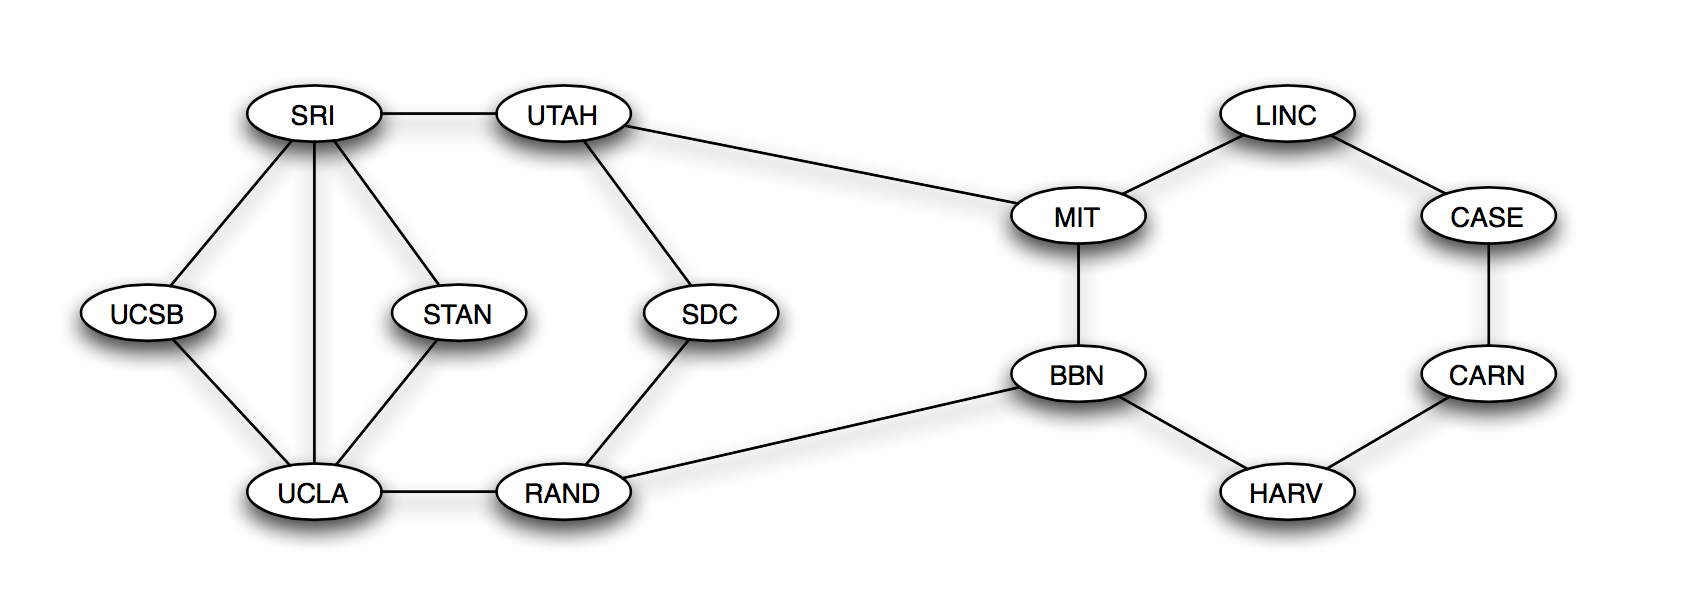
\includegraphics[scale=.4]{img/arpanetdec1970_graph.png}
	\caption{Grafo di ARPANET nel Dicembre 1970}
	\label{arpanet_graph}
\end{figure}
Il grafo di ARPANET mostrato in precedenza è un esempio di \textit{\textbf{communication network}}, i cui nodi sono computer o altri dispositivi capaci di inviare messaggi mentre gli archi rappresentano i collegamenti diretti lungo i quali tali messaggi possono viaggiare. Ma questo è solamente uno dei tipi di rete che possiamo avere.\\
Le \textit{\textbf{social network}} i cui nodi sono persone o gruppi di persone, ed i cui archi rappresentano un tipo di interazione (amicizia, inimicizia, ecc.), sono reti massive che al giorno d'oggi comprendono gran parte della popolazione mondiale, come ad esempio le reti di Facebook e Twitter.\\
Le \textit{\textbf{information network}} sono reti che rappresentano il mondo dell'informazione, i cui nodi sono le fonti di informazione e gli archi rappresentano collegamenti logici come riferimenti, citazioni identificati da hyperlink. A tale categoria appartiene il grafo del Web, così come la rete di documenti di Wikipedia.\\
Le \textit{\textbf{dependency network}}, che descrivono le dipendenze esistenti in una collezione di oggetti. Ne sono esempi reti di dipendenze tra task, per cui sono stati sviluppati molti lavori, applicati anche in altri campi come lo studio del sistema immunitario e delle reti semantiche.\\
I grafi mostrano la loro grande utilità anche nelle \textit{\textbf{transportation network}}, reti i cui nodi sono luoghi geografici ed i cui archi sono le linee stradali, ferroviarie o aeree che li collegano. Questo tipo di rete è stata di grande importanza nello sviluppo di concetti ed algoritmi su grafi, infatti molta della terminologia deriva dal mondo dei trasporti.\\
Quindi, come si evince dai vari tipi di network descritte finora, i grafi sono uno strumento potente che trova applicazione nelle realtà più disparate, partendo dalla matematica ed informatica, fino ad arrivare agli studi della sociologia, biologia, linguistica, chimica e fisica. Ed è proprio l'ultimo ambito ad interessare questo lavoro di tesi: la \textit{fisica statistica} è una branca della fisica che utilizza metodi della teoria delle probabilità e statistici, ed in particolare gli strumenti matematici usati per gestire grandi popolazioni ed approssimazioni, per la risoluzione di problemi fisici. Può descrivere una grande varietà di campi dotati di una natura stocastica intrinseca. Le sue applicazioni coinvolgono problemi nel campo della fisica, biologia, chimica, neurologia e scienze sociali.\\
Lo scopo finale per cui nasce la fisica statistica, in particolare la meccanica statistica, è quello di fornire strutture e strumenti per mettere in relazione proprietà microscopiche di atomi e molecole individuali rispetto a proprietà del materiale che possono essere osservate ad occhio nudo. Spiegando ad esempio la termodinamica come il risultato naturale di statistica, meccanica classica e meccanica quantistica al livello microscopico: il grafo riesce a modellare le particelle del sistema su cui agisce la dinamica del processo fisico.


\section{Modello di Ising}\label{sec:ising}
Il modello di Ising è un classico problema combinatoriale della fisica statistica, studiato per la prima volta da Ernest Ising nel 1920. Tale modello è interessato alla fisica delle transizioni di fase, che occorrono quando un piccolo cambiamento nei parametri, come temperatura o pressione, causa un grande cambiamento qualitativo nello stato del sistema. Le transizioni di fase sono comuni nella fisica, come ad esempio nel fenomeno del ferromagnetismo.\\
Uno degli scopi principali del modello di Ising è spiegare come interazioni di breve raggio tra le componenti del sistema siano in grado di dare luogo a comportamenti correlati di lungo raggio e, quindi, di predire in un certo senso il potenziale per una transizione di fase. Tale modello trova applicazione in molti ambiti, in generale in tutti quegli ambiti dove si studia il comportamento cooperativo di grandi sistemi: tali applicazioni sono possibili perché il modello di Ising può essere formulato come un problema matematico.\\
Una semplice definizione matematica del modello di Ising è data in \cite{cipra1987introduction} e in \cite{jerrum1993polynomial}: consideriamo una collezione di siti $\lbrack n \rbrack = \lbrace 0, 1, \cdots, n-1 \rbrace$, in cui ogni coppia $i, j$ ha associata un’energia di interazione $V_{ij}$. Nella maggior parte dei casi di interesse fisico, l’insieme E di coppie con energia di interazione non nulla forma un \textit{regular lattice graph} $([n], E)$: detto anche \textit{mesh graph} o \textit{grid graph}, è un grafo la cui rappresentazione grafica sul piano forma delle tassellature regolari.\\
Il primo passo del modello è quello di assegnare ad ogni sito \textit{i} una variabile $\sigma_i$, detta \textbf{spin}, con $i=1, \dots, n$. Le variabili $\sigma_i$ possono assumere solo due valori, $\sigma_i = \pm 1$, che si possono definire come gli \textit{stati} dei siti.\\
Una \textbf{configurazione} $\sigma$ del sistema è un assegnamento di spin positivi $\left( \sigma_i = 1 \right)$ o negativi $\left( \sigma_i = 1 \right)$ ad ogni sito $i \in \lbrack n \rbrack$.\\
L'\textit{energia} di una configurazione è data dall’Hamiltoniana del sistema: nella fisica matematica, tale quantità governa le dinamiche del sistema. Per il modello di Ising, l’Hamiltoniana è definita sotto un’assunzione ben precisa: si assume che solo le interazioni di breve raggio e con i siti più vicini e le interazioni dei siti con un ``campo esterno'' contribuiscono al livello di energia del sistema. Pertanto, per ogni configurazione $\sigma = (\sigma_1, \dots, \sigma_n)$ si ha:\\
\begin{equation}
H(\sigma) = - \sum_{\lbrace i,j \rbrace \in E}{V_{ij}\sigma_i\sigma_j} - B \sum_{k\in\lbrack n \rbrack}{\sigma_k}
\end{equation}
in cui la prima sommatoria varia su tutte le coppie di vicini nel lattice graph mentre la seconda varia su tutti i siti del sistema. $V_{ij}$ e B sono parametri associati rispettivamente alle interazioni dei vicini ed alle interazioni con il campo esterno.\\
Nel caso in cui tutte le energie di interazione siano non negative, tale sistema modella il comportamento di un \textit{ferromagnete}: una configurazione ``'magnetizzata' (con la maggior parte di coppie di siti vicini aventi $\sigma_i = \sigma_j$), ha un livello di energia più basso rispetto ad una configurazione non magnetizzata. Il parametro B corrisponde alla presenza di un ``campo magnetico esterno''.
\subsection{Partition Function}
La funzione di partizione è senza alcun dubbio l'oggetto di maggior rilievo introdotto dalla meccanica statistica. La si ottiene dall'esponenziazione dell'Hamiltoniana e sommando su tutte le possibili configurazioni $\sigma$, cioè su $2^n$ possibili assegnamenti di valori $\pm1$ alle $n$ variabili $(\sigma_1, \dots, \sigma_n)$:
\begin{equation}
	Z = Z(V_{ij}, B, \beta) = \sum_{\sigma}{exp(-\beta H(\sigma))}.
\end{equation}
Nell'ambito della meccanica statistica, solitamente $\beta = 1 / kT$, dove $k$ è la costante di Boltzmann e T è la temperatura $(\beta > 0)$.\\
La partition function è utilizzata come ``denominatore'' nel calcolo delle probabilità. In particolare, la probabilità che il sistema si trovi in una specifica configurazione $\sigma$ è data dalla formula
\begin{equation}
	P(\sigma) = \frac{e^{-\beta H(\sigma)}}{Z}
\end{equation}
Il segno negativo apporta una maggiore probabilità agli stati con energia più bassa. Valori bassi di $\beta$, corrispondenti ad alta temperatura, tendono ad ``appiattire'' la distribuzione, rendendo così tutte le configurazioni equiprobabili o quasi. Alti valori di $\beta$, corrispondenti a bassa temperatura, tendono ad apportare maggiore probabilità agli stati con energia minore.\\
È possibile ottenere, a partire dalla partition function Z, due quantità altrettanto importanti, la \textit{mean energy} $\epsilon = -\partial(ln Z)/\partial\beta$ ed il \textit{mean magnetic moment} $\mathcal{M} = \beta^{-1}\partial(ln Z)/\partial\beta$.
\section{Cenni di probabilità e statistica}
Di seguito vengono riportati concetti e definizioni utili alla comprensione di questo lavoro di tesi (per maggiori dettagli consultare \cite{grinstead2012introduction}).\\
\paragraph{Spazio delle probabilità.} Tripla $(\Omega, F, P)$, dove $\Omega$ è lo \textit{spazio campionario}, cioè l'insieme dei possibili esiti (o \textit{outcome}), $F$ è l'insieme degli eventi, mentre $P : \mathcal{F} \rightarrow [0, 1]$ è una funzione che assegna probabilità ad eventi.\\
\paragraph{Variabile aleatoria.} Definita su uno spazio di probabilità, esprime il valore numerico di un outcome di un evento. Una variabile aleatoria \textit{X} è una funzione definita sullo spazio degli outcome $\Omega$, ed associa ad ogni elemento di $\Omega$ un valore in $\mathcal{R}$.
Sia \textit{X} una variabile casuale che rappresenta il valore degli outcome di un certo evento e si assuma che tale evento possa avere solo un numero finito di possibili outcome. Sia $\Omega$ lo spazio campionario dell'esperimento. Una \textit{funzione di distribuzione} per \textit{X} è una funzione \textit{p} di valori reali il cui dominio è $\Omega$ e che soddisfa $p(\omega) \geq 0$ e $\sum{p(\omega)} = 1$, con $\omega \in \Omega$.\\
Per ogni sottoinsieme \textit{E} di $\Omega$, definiamo la \textit{probabilità} di \textit{E} come
\begin{equation}
	P(E) = \sum_{\omega \in E}{p(\omega)}.
\end{equation}
La funzione $p(\omega)$ è la \textbf{distribuzione di probabilità} della variabile aleatoria \textit{X}.
\paragraph{Valore atteso.} Sia \textit{X} una variabile casuale discreta con spazio campionario $\Omega$ e funzione di distribuzione $p(x)$. Il \textit{valore atteso E(X)} è definito come
\begin{equation}
	E(X) = \sum_{x\in \Omega} x p(x)
\end{equation}
a patto che tale sommatoria converga (altrimenti X non avrebbe valore atteso).
Di solito, il valore atteso è anche chiamato \textit{media}, ed è indicato con il simbolo $\mu$. Alcune delle principali proprietà di cui gode il valore atteso sono riportate di seguito:
\begin{itemize}
	\item Siano $X$ ed $Y$ due variabili aleatorie con valori attesi finiti, allora $E(X+Y) = E(X) + E(Y)$
	\item Sia X una variabile aleatoria con valore atteso finito e sia $c$ una costante, allora $E(cX) = cE(X)$
	\item Siano X e Y due variabili aleatorie indipendenti, allora $E(X\cdot Y) = E(X) \dot E(Y)$.
\end{itemize}
\paragraph{Varianza.} Sia \textit{X} una variabile casuale con valore atteso $\mu = E(X)$. Allora la \textit{varianza} di X, indicata con $V(X)$, o con $\sigma^2$, è pari a
\begin{equation}
	V(X) = E((X - \mu^2)).
\end{equation}
La varianza può essere anche scritta come
\begin{equation}
	V(X) = \sum_x {(x - \mu^2)p(x)}.
\end{equation}
Una utile alternativa al calcolo della varianza è data dal seguente teorema: \textit{sia X una variabile casuale con} $E(X) = \mu^2$, \textit{allora} $V(X) = E(X^2) - \mu^2$. Per maggiori dettagli riguardati la prova di tale teorema, consultare pagina 258 di \cite{grinstead2012introduction}.\\
Alcune importanti proprietà della varianza:
\begin{itemize}
	\item Sia \textit{X} una variabile casuale e $c$ una costante, allora $V(cX) = c^2V(X)$
	\item Siano $X$ ed $Y$ due variabili casuali indipendenti, allora $V(X+Y) = V(X) + V(Y)$.
\end{itemize}
\paragraph{Disuguaglianza di Chebyshev.} \label{chebyshev} Sia \textit{X} una variabile casuale con valore atteso finito $\mu$ e varianza non negativa finita $\sigma^2$. Allora per qualsiasi numeri reale $k > 0$ si ha che
\begin{equation}
	Pr(|X - \mu| \geq k) \leq \frac{\sigma^2}{k^2}.
\end{equation}
Tale disuguaglianza garantisce che in qualsiasi distribuzione di probabilità, quasi tutti i valori siano vicini alla media.
\section{Processi Markoviani}\label{sec:markovproc}
Di seguito sono introdotti i concetti alla base delle catene di Markov (consultare \cite{levin2009markov} per maggiori dettagli).\\
Una catena di Markov finita è un processo che si muove tra gli elementi di un insieme finito $\Omega$ nel seguente modo: se si suppone di trovarsi in $x \in \Omega$, allora la prossima posizione è scelta in accordo ad una distribuzione di probabilità fissata $P(x, \cdot)$. Più precisamente, una sequenza di variabili casuali $(X_0, X_1, \dots)$ è una \textbf{catena di Markov con spazio degli stati $\Omega$ e matrice di transizione P} se per tuttu gli $x,y \in \Omega$, per tutti i $t \geq 1$, e per tutti gli eventi $H_{t-1} = \bigcap_{s=0}^{t-1}{X_s = x_s}$ che soddisfano $Pr(H_{t-1} \cap {X_t = x}) > 0$, si ha
\begin{equation}
	Pr(X_{t+1} = y | H_{t-1} \cap {X_t = x}) = Pr(X_{t+1} = y | X_t = x) = Pr(x, y).
	\label{pr_xy}
\end{equation}
L'equazione \ref{pr_xy}, nota come \textit{proprietà di Markov}, sta a significare che la probabilità condizionale di procedere dallo stato $x$ allo stato $y$ è la stessa, non importa quale sia la lunghezza degli stati $x_0, \dots, x_{t-1}$ che precedono lo stato corrente $x$. 
\subsection{Irriducibilità e periodicità}
Una catena di Markov P è detta \textbf{irriducibile} se, per qualsiasi coppia di stati $x, y \in \Omega$, esiste un intero \textit{t} tale che $P^t(x, y) > 0$. L'affermazione sta ad indicare che è possibile andare da uno stato in un qualsiasi altro stato utilizzando solo transizioni di probabilità positive.\\
Sia $\mathcal{T}(x) := {t \geq 1 : P^{t}(x,x) > 0}$ l'insieme di volte in cui è possibile per la catena ritornare nella posizione iniziale $x$. Il \textbf{periodo} di $x$ è definito come il \textit{massimo comune divisore (gcd)} di $\mathcal{T}(x)$.\\
\paragraph{Lemma.} \textit{Se P è irriducibile, allora gcd($\mathcal{T}(x)$) = gcd($\mathcal{T}(y)$)} $\forall x, y \in \Omega$.\\
Data una catena irriducibile, il periodo della catena è definito come il periodo che è comune a tutti gli stati. La catena sarà detta \textit{aperiodica} se tutti gli stati hanno periodo 1, altrimenti \textit{periodica}.
\paragraph{Proposizione.} \textit{Se P è aperiodica ed irriducibile, allora vi è un intero r t.c.} $P^r(x, y) > 0 \forall x, y \in \Omega$.\\
Una catena di Markov finita (con spazio degli stati $\Omega$ finito), \textit{irriducibile} ed \textit{aperiodica} è detta \textbf{ergodica}.
\subsection{Distribuzione stazionaria}\label{ssec:stazdist}
Sia $\pi$ una distribuzione di probabilità. Se tale distribuzione soddisfa
\begin{equation}
	\pi = \pi P
\end{equation}
allora $\pi$ è detta \textit{distribuzione stazionaria} della catena di Markov. tale distribuzione può essere riscritta anche per i singoli elementi della catena:
\begin{equation}
	\pi(x) = \sum_{x\in \Omega}{\pi(x)P(x, y)} \forall x,y \in \Omega.
\end{equation}
Il risultato ben noto, che si ottiene dalla teoria dei processi Markoviani è che se la catena in questione è ergodica, allora la distribuzione stazionaria è \textit{unica}.\\
Una catena di Markov è detta \textit{reversibile} se
\begin{equation}
	\pi(x)P(x,y) = \pi(y)P(y,x) \forall x,y \in \Omega.
	\label{revchain}
\end{equation}
Quindi, data una catena $(X_t)$ che soddisfa \ref{revchain} ed ha una distribuzione stazionaria iniziale, allora la distribuzione di $(X_0, X_1, \dots, X_n)$ è la stessa di $(X_n, X_{n-1}, \dots, X_0)$.\\
Un risultato di grande importanza è il \textit{teorema della convergenza}: tale teorema prova che una catena di Markov irriducibile ed aperiodica converge alla sua distribuzione stazionaria.\\
Prima di enunciare il problema, però, è necessaria la definizione di \textit{total variation distance}: siano $\pi$ e $\mu$ due distribuzioni di probabilità sullo stesso spazio campionario $\Omega$, allora la total variation distance è definita come
\begin{equation}
	\|\pi - \mu\| = max_{A\subset\Omega}|\pi(A) - \mu(A)| = \frac{1}{2}\sum_{x\in\Omega}{|\pi(x) - \mu(x)|}.
\end{equation}
Si enuncia ora, il \textbf{teorema della convergenza}:
\paragraph{Teorema.} \textit{Si supponga che P sia irriducibile ed aperiodica, con distribuzione stazionaria $\pi$. Allora esistono due costanti $\alpha \in (0,1) e C > 0 t.c.$}
\begin{equation}
	max_{x\in\Omega}\|P^t(x,\cdot) - \pi\| \leq C\alpha^t.
	\label{convth}
\end{equation}
Per la dimostrazione e maggiori dettagli consultare \cite{levin2009markov} (pag. 52).
\subsection{Catena di Markov Monte Carlo}
Data una matrice di transizione irriducibile \textit{P}, vi è un'unica distribuzione stazionaria $\pi$ che soddisfa $\pi = \pi P$, come affermato nella sezione precedente.\\
Si consideri ora il problema inverso: data una distribuzione di probabilità $\pi$ su $\Omega$, è possibile trovare una matrice di transizione \textit{P} per cui $\pi$ è la distribuzione stazionaria? \cite{levin2009markov} fornisce un esempio pratico per capire come risolvere tale problema.\\
Il \textit{campione casuale} da un insieme finito $\Omega$ è definito come una selezione uniformemente casuale da $\Omega$; una selezione tale che ogni elemento ha la stessa probabilità $1/|\Omega|$ di essere scelto.\\
Sia ${1, 2, \dots, q}$ un insieme di \textit{colori}. Un \textit{proper q-coloring} di un grafo $G=(V, E)$ è un assegnamento di colori ai vertici di V, con il vincolo che nodi vicini non debbano avere lo stesso colore. Per alcune tipologie di grafo, come ad esempio gli alberi, esistono semplici metodi ricorsivi che generano una colorazione casuale; per altri grafi, invece, risulta più difficile. un approccio consiste nell'utilizzare le catene di Markov per campionare: supponiamo che $(X_t)$ sia una catena con spazio degli stati $\Omega$ e con una distribuzione stazionaria uniforme su $\Omega$. Grazie al teorema della convergenza enunciato in \ref{convth}, $X_t$ è approssimativamente uniformemente distribuita quando $t$ è grande.\\
tale metodo di campionamento a partire da una data distribuzione di probabilità è chiamato \textit{\textbf{Catena di Markov Monte Carlo}}. Si supponga che $\pi$ sia una distribuzione di probabilità su $\Omega$. se + possibile costruire una catena di Markov $(X_t)$ con distribuzione stazionaria $\pi$ allora, per $t$ grande abbastanza si ha che la distribuzione di $X_t$ è vicina a $\pi$.
\section{Algoritmi di approssimazione}\label{sec:approxalgo}
Un \textit{\textbf{$\alpha$-approximation algorithm}} per un dato problema è un algoritmo con tempo di esecuzione polinomiale che, per tutte le istanze del problema, produce una soluzione il cui valore è entro un fattore $\alpha$ del valore della soluzione ottima.\\
Dato un $\alpha$-approximation algorithm, $\alpha$ è la \textit{performance} garantita dell'algoritmo. In letteratura è spesso anche chiamato \textit{rapporto di approssimazione} o \textit{fattore di approssimazione}.\\
Un \textit{\textbf{polynomial time approximation scheme}} è una famiglia di algoritmi ${A_\epsilon}$, in cui vi è un algoritmo per ogni $\epsilon > 0$ tale che $A_\epsilon$ è un $()1+\epsilon$-approximation algorithm (per problemi di minimizzazione) o un $(1-\epsilon)$-approximation algorithm (per problemi di massimizzazione).\\
Oltre a queste due definizioni riportate in \cite{williamson2011design}, è interessante fornire le definizioni tratte dal paper di riferimento di questo lavoro di tesi \cite{jerrum1993polynomial}:\\
dati numeri reali non negativi $a, \tilde{a}, \epsilon$, si dice che $\tilde{a}$ approssima $a$ in un range $(1+\epsilon)$ se
\begin{equation}
	a(1+\epsilon)^{-1} \leq \tilde{a} \leq a(1+\epsilon).
\end{equation}
Sia \textit{f} una qualsiasi funzione che mappa istanze del problema in numeri reali. Un \textit{\textbf{randomised approximation scheme}} per $f$ è un algoritmo probabilistico che, quando presentato con un'istanza $x$ ed un numero reale $\epsilon \in (0,1]$, restituisce un numero che, con alta probabilità, approssima $f(x)$ in un range $(1+\epsilon)$. Il risultato di tale algoritmo, però, non deve essere ottenuto solo con \textit{alta affidabilità}, ma anche \textit{efficientemente}. In accordo a ciò, si definisce un approximation scheme \textit{\textbf{fully polynomial}} se il suo tempo di esecuzione è polinomiale in $\epsilon^{-1}$ e nella taglia dell'istanza $x$ del problema.

%%%%%%%%%%%%%%%%%%%%%%%%%%%%%%%%%%%%%%%%%%%
\chapter{Logit Dynamics}
In questo capitolo si descrive la \textit{Logit dynamics}, introdotta per la prima volta da Blume in \cite{blume1993statistical}. Si evidenziano le sue proprietà e le sue motivazioni. Maggiori dettagli in \cite{ferraioli2012logit}.
\section{Definizione}
Si consideri un gioco strategico $\mathcal{G} = ([n], S_1, \dots, S_n, u_1, \dots, u_n)$, in cui $[n] = {1, \dots, n}$ è un insieme finito di giocatori, $S_i$ è l'insieme finito di strategie per il giocatore $i, S = S_1 \times \cdots \times S_n$ è l'insieme dei profili di strategie ed $u_i: S \rightarrow \mathcal{R}$ è la funzione utilità del giocatore $i \in [n]$.\\
La \textit{Logit dynamics} per un gioco $\mathcal{G}$ procede come segue, ad ogni step:
\begin{enumerate}
	\item si sceglie un giocatore $i \in [n]$ a caso;
	\item sia ggiorna la strategia del giocatore $i$ in accordo alla \textit{logit update rule} con parametro $\beta \geq 0$ sull'insieme $S_i$ delle sue strategie. Cioè. la dinamica sceglie una strategia $s \in S_i$ con probabilità
	\begin{equation}
		\sigma_i (s|x) = e^{\beta u_i (s, x_{-i})}/Z_i(x),
		\label{sigmai}
	\end{equation}
	in cui $x = (x_1, \dots, x_n) \in S$ è il profilo di strategie corrente, $\beta \geq 0$ e
	\begin{equation}
		Z_i(x) = \sum_{z\in S_i}{e^{\beta u_i (s, x_{-i})}}
	\end{equation}
	è il fattore di normalizzazione.
\end{enumerate}

Il parametro $\beta$ indica il \textit{livello di razionalità} del sistema; pertanto, quando $\beta = 0$ il giocatore \textit{i} sceglie la sua strategia in maniera casuale, mentre con $\beta > 0$, la probabilità è influenzata dalle strategie che permettono un \textit{payoff} maggiore, e per $\beta \rightarrow \infty$ il giocatore sceglie la sua \textit{best response}. Inoltre, bisogna notare che la probabilità $\sigma_i (s|x)$ non dipende dalla strategia $x_i$ attualmente adottata dal giocatore $i$.
Formalmente, la dinamica può essere definita anche nel seguente modo.
\paragraph{Definizione 3.1.1} \textit{Sia $\mathcal{G} = ([n], \mathcal{S}, \mathcal{U})$ un gioco strategico e sia $\beta \geq 0$. La Logit dynamics per $\mathcal{G}$ è la catena di Markov $\mathcal{M}_{\beta} = ({X_t}_{t \in N}, S, P)$ dove $S = S_1 \times \cdots \times S_n$ e}
\begin{equation}
	P(x, y) = \frac{1}{n} \cdot 
	\begin{cases}
	\sigma_i(s_i|x), & \text{se}\ y_{-i} = x_{-i} \text{ed}\ y_i \neq x_i\\
	\sum_{i=1}^{n}{\sigma_i(s_i|x)}, & \text{se}\ x = y\\
	0, & \text{altrimenti}
	\end{cases}
	\label{ergmc}
\end{equation}
\textit{con $\sigma_i(s_i|x)$ definita in \ref{sigmai}.}
Come sarà mostrato nella sezione \ref{ssec:ergod}, la catena di Markov descritta in \ref{ergmc} è ergodica. Pertanto, indipendentemente dallo stato di partenza, la distribuzione della catena al tempo \textit{t} convergerà alla \textit{distribuzione stazionaria $\pi$} man mano che \textit{t} tende ad infinito.\\
Si consideri ora un \textit{potential game}. Per tale gioco, la distribuzione stazionaria è la ben nota \textit{Gibbs measure}.
\paragraph{Teorema 3.1.1} \textit{Se $\mathcal{G} = ([n], \mathcal{S}, \mathcal{U})$ è un potential game con funzione potenziale $\Phi$, allora la catena di Markov descritta in \ref{ergmc} è reversibile e la sua distribuzione stazionaria è data dalla Gibbs measure}
\begin{equation}
	\pi(x) = \frac{1}{Z}{e^{\beta\Phi(x)}},
	\label{gibbsm}
\end{equation}
\textit{con $Z = \sum_{y\in S}{e^{\beta\Phi(y)}}$ è la costante di normalizzazione.}
\section{Proprietà}
Si analizzano ora alcune proprietà della \textit{Logit dynamics} utili alla comprensione di questo lavoro di tesi. Per ulteriori proprietà e dettagli consultare \cite{ferraioli2012logit}.
\subsection{Ergodicità} \label{ssec:ergod}
È semplice vedere come la catena di Markov descritta in \ref{ergmc} sia ergodica. Siano $x = (x_1, \dots, x_n)$ ed $y = (y_1, \dots, y_n)$ due profili e sia $z=(z^0, \dots, z^n)$ un \textit{cammino} di profili dove $z^0 = x, z^n = y$ e $z^i=(y_1, \dots, y_i, x_{i+1}, \dots, x_n)$ per $i=1, \dots, n-1$. La probabilità che la catena, iniziando in $x$, si trovi in $y$ dopo $n$ passi è
\begin{equation}
	P^n(x,y) = P^n(z^0, z^n) \geq P^{n-1}(z^0, z^{n-1})P(z^{n-1}, z^n),
\end{equation}
e, ricorsivamente
\begin{equation}
	P^n(x,y) \geq \prod_{i=1}^{n}{P(z^{i-1}, z^i)} > 0,
\end{equation}
dove l'ultima disuguaglianza deriva da \ref{ergmc}.

\subsection{Logit dynamics e Glauber dynamics}
In un \textit{potential game}, la \textit{Logit dynamics} è equivalente alla ben nota \textit{Glauber dynamics}.\\
Sia $S = S_1 \times \cdots S_n$ uno spazio degli stati e sia $\mu$ una distribuzione di probabilità su $S$, allora la \textit{Glauber dynamics} per $\mu$ procede come segue:\\
da un profilo $x \in S$ si sceglie un giocatore $i \in [n]$ in maniera casuale e si modifica la sua strategia in $y \in S_i$ con probabilità $\mu$ condizionata dagli altri giocatori che sono in $x_{-i}$
\begin{equation}
	\mu(y|x_{-i}) = \frac{\mu(x_{-i}, y)}{\sum_{z\in S_i}{\mu(x_{-i}, z)}}.
\end{equation}
È facile vedere come la catena di Markov definita dalla \textit{Glauber dynamics} sia irriducibile, aperiodica e reversibile, con distribuzione stazionaria $\mu$. Quando $\mathcal{G}=([n], \mathcal{S}, \mathcal{U})$ è un \textit{potential game} con funzione potenziale $\Phi$, la \textit{Logit dynamics} definisce la stessa catena di Markov che la \textit{Glauber dynamics} definisce per la \textit{Gibbs distribution} $\pi$ in \ref{gibbsm}.
In accordo a quanto appena detto, la \textit{Logit dynamics} per un \textit{potential game} e la \textit{Glauber dynamics} per la \textit{Gibbs distribution} sono due modi di guardare la stessa catena di Markov. Grazie a tale analogia, ci si può riferire alla terminologia utilizzata dai fisici per indicare le quantità coinvolte, in particolare, il parametro $\beta$ è detto \textit{inverse temperature} ed il fattore di normalizzazione $Z$ della \textit{Gibbs distribution} \ref{gibbsm} è detto \textit{partition function}.
\section{Movitazioni}
Nel lavoro introduttivo alla \textit{Logit dynamics} \cite{blume1993statistical}, Blume sottolinea che essa evidenzia due concetti chiave del comportamento strategico: \textit{lock-in} e \textit{bounded rationality}.\\
La prima proprietà stabilisce che, una volta che un giocatore effettua una scelta, si lega ad essa per qualche tempo: assumendo che tale regola valga nella realtà, giustifica una regola per la scelta di una strategia che tiene conto solamente delle strategie attualmente giocate dagli altri partecipanti e non le strategie che sono state precedentemente scelte. Questo è esattamente ciò che la \textit{Logit update rule} fa in \ref{sigmai}.\\
La seconda proprietà interviene nella dinamica in due modi: nel comportamento \textit{miopico} dei giocatori che considerano solo il guadagno attuale e non una prospettiva di guadagni futuri e l'\textit{informazione limitata} che tali giocatori hanno. È evidente che la \textit{Logit update rule} in \ref{sigmai} considera tali aspetti. Inoltre, poiché la dinamica descrive una catena di Markov, l'evoluzione del sistema viene trattata in maniera chiara e semplice, permettendo analisi avanzate attraverso gli strumenti forniti dalla teoria dei processi markoviani (alcuni descritti in \ref{sec:markovproc}). Non essendoci restrizioni circa la struttura dei giochi o la loro funzione utilità, tali dinamiche possono essere applicate ad ogni sistema di interesse.\\
Un'altra caratteristica, che rende tali dinamiche appetibili, è la forte presenza di \textit{probabilità} e \textit{casualità}. L'approccio probabilistico della \textit{Logit dynamics} è motivato anche dalla volontà di modellare sistemi complessi, intrinsecamente casuali e, pertanto, descrivibili solo attraverso modelli probabilistici.\\
La \textit{Logit dynamics}, quindi, soddisfa una serie di proprietà interessanti che motivano il loro impiego come modello utilizzato per studiare l'evoluzione dei giochi.
\section{Alcuni Esperimenti}
In letteratura sono presenti diversi esperimenti atti a paragonare le predizioni della \textit{Logit dynamics} con dati reali.\\
McKelvey e Palfrey, in \cite{mckelvey1993quantal}, si focalizzano su esperimenti che coinvolgono giochi con due persone in cui vi è un unico equilibrio Nash. I dati reali sono stati raccolti da esperimenti che sono stati eseguiti in più di trent'anni.\\
Per ogni esperimento, è stata calcolata la stima a \textit{maximum likelihood} del parametro $\beta$ ed è stato analizzato quanto bene il modello approssimi i dati.
I risultati mostrano che la \textit{Logit dynamics} predice deviazioni sistematiche dall'equilibrio Nash. Ciononostante, gli autori fanno notare che, sebbene ci sia consistenza con il parametro $\beta$ negli esperimenti fatti, vi siano alcuni aspetti dei dati reali che non trovano spiegazione in tale dinamica.\\
Cameter et al. \cite{ho2007self} considerano sette giochi e stimano il parametro $\beta$ utilizzando il $70\%$ dei soggetti, ed utilizzano tale stima per predire il comportamento del rimanente $30\%$ dei soggetti. Mentre, in un altro test, utilizzano sei giochi per stimare $\beta$ ed utilizzano tali stime sul settimo gioco. I risultati mostrano che ci sono giochi in cui le predizioni della \textit{Logit dynamics} sono paragonabili ai risultati di dinamiche più forti che, però, sono intrattabili analiticamente e si suppone che non convergeranno mai in qualsiasi gioco.

%%%%%%%%%%%%%%%%%%%%%%%%%%%%%%%%%%%%%%%%%%%
\chapter{Il lavoro di Jerrum e Sinclair}
Questo capitolo focalizza l'attenzione sul lavoro che ha gettato le fondamenta per lo sviluppo del e su cui si basa questa tesi e tanti altri lavori. L'articolo di cui si parla è ``\textit{Polynomial-time approximation algorithms for the Ising model}'', scritto da Mark Jerrum ed Alistair Sinclair nel 1993 \cite{jerrum1993polynomial}.\\
In breve, \cite{jerrum1993polynomial} presenta un algoritmo randomizzato che calcola la partition function di un sistema di Ising ferromagnetico qualunque, con grado di accuratezza arbitrario. Il tempo di esecuzione di tale algoritmo è polinomiale nella taglia del sistema (i.e. il numero di siti) e variabile in base ad un parametro che controlla l'accuratezza del risultato.
L'algoritmo si basa su una simulazione Monte Carlo di una catena di Markov ergodica opportunamente definita. Si può già anticipare che gli stati della catena non sono, come accade di solito, configurazioni di spin di Ising, ma spanning subgraph del grafo di interazione del sistema. Le performance dell'algoritmo sono garantite da prove rigorose e poggiano sulla proprietà di \textit{rapidly mixing} della catena di Markov: converge alla sua distribuzione d'equilibrio in un numero \textit{polinomiale} di passi.\\
Si prosegue con l'analisi dettagliata dell'algoritmo proposto da Jerrum e Sinclair, descrivendo prima il modo con cui si trasforma il modello di Ising in un nuovo dominio, in cui le configurazioni sono spanning subgraph del grafo di interazione; prosegue con la costruzione di un \textit{fully polynomial randomised approximation scheme (fpras)} per il calcolo della partition function ed infine analizzando la catena di Markov definita sulle nuove configurazioni.\\
Nei capitoli successivi, l'algoritmo proposto verrà identificato come ``\textit{algoritmo naive}''.
\section{Spins world e Subgraphs world}
L'obiettivo è costruire un algoritmo per il seguente problema:
\textbf{Istanza}: una matrice reale simmetrica $(V_{ij} : i,j \in [n])$ delle energie di interazione, un numero reale B che rappresenta il campo esterno ed un numero reale positivo $\beta$.
\textbf{Output}: la partition function
\begin{equation}
	Z = Z(V_{ij}, B, \beta) = \sum_{\sigma}{exp(-\beta H(\sigma))},
	\label{partf}
\end{equation}
Dove l'Hamiltoniana $H(\sigma)$ è data da
\begin{equation}
	H(\sigma) = - \sum_{\{i,j\}\in E}{V_{ij}\sigma_i\sigma_j} - B\sum_{k\in [n]}{\sigma_k}
	\label{hamilt}
\end{equation}
ed E è l'insieme di coppie non ordinate ${i, j}$ con $V_{ij} \ne 0$.\\
Tale algoritmo tratta il caso \textit{ferromagnetico} del modello di Ising, che è caratterizzato da energie di interazione $V_{ij}$ non negative. È importante tenere a mente che piuttosto di calcolare \textit{esattamente} la partition function, si preferisce approssimarla.\\
Una strategia, rivelatasi molto utile per problemi di questo tipo, prevede la simulazione di una catena di Markov opportuna. Un'applicazione diretta di questa strategia alla partition function di Ising procederebbe come segue: si considerino le configurazioni del sistema di Ising, cioè i $2^n$ possibili vettori di spin $\sigma \in {-1, +1}^n$, come gli stati della catena di Markov. Si scelgano poi le probabilità di transizione tra gli stati così da rendere la catena \textit{ergodica} e quindi, nella distribuzione stazionaria, la probabilità di essere nello stato $\sigma$ è $Z^{-1}exp(-\beta H(\sigma))$. Un modo ragionevole per raggiungere ciò, spesso utilizzato, è permettere che le transizioni occorrano tra configurazioni di sping che differiscano in una sola componente, e scegliere le probabilità di transizione in accordo alla regola di Metropolis \cite{gelatt1983optimization}. Se la catena di Markov risultante è \textit{rapidly mixing}, cioè se converge rapidamente alla distribuzione stazionaria indipendentemente dalla scelta dello stato iniziale, allora può essere usata efficacemente per campionare le configurazioni $\sigma$ da una distribuzione che è vicina alla distribuzione stazionaria. Raccogliendo sufficienti campioni di configurazioni, usando differenti valori di B e $\beta$, dovrebbe essere possibile stimare la partition function $Z$ con buona accuratezza.\\
Purtroppo, la catena di Markov così descritta (lo \textit{spin-world process}) non è rapidly mixing. È ben noto che i sistemi ferromagnetici di Ising esibiscono tipicamente una transizione di fase ad un certo valore del parametro $\beta$, per valori al di sopra del punto critico, il sistema si stabilizza in uno stato in cui vi è una preponderanza di spin di uno o l'altro segno. transizioni tra gli stati con maggioranza di +1 e stati con maggioranza di -1 occorrono raramente, semplicemente perché la distribuzione stazionaria assegna un peso totale di basso valore alle configurazioni con spin bilanciati.\\
Il problema causato dall'assenza di \textit{rapid mixing} nello \textit{spin-world process} può essere aggirato simulando una catena di Markov differente: il \textit{subgraphs-world process}. Sebbene le due catene di Markov siano strutturalmente differenti, ed inoltre, il \textit{subgraphs-world process} non abbia alcun significato fisico, quest'ultimo ha una forte connessione con la \textit{partition function} del modello di Ising e, cosa fondamentale nell'applicazione corrente, è \textit{rapidly mixing}.\\
Tale processo sarà descritto in dettaglio nella sezione \ref{sec:swp}.\\\\
Un sottografo si dice \textit{spanning} se include tutti i vertici del grafo ``genitore'' (in generale gli \textit{spanning subgraph} non sono connessi). Le configurazioni del \textit{subgraph-world} sono \textit{spanning subgraph} del grafo di interazione $([n], E)$. Per semplificare la notazione, siano
\begin{equation}
	\lambda_{ij} = tanh \beta V_{ij}
	\label{lamij}
\end{equation}
\begin{equation}
	\mu = tanh B \beta
	\label{mu}
\end{equation}
Ad ogni configurazione $X \subseteq E$ è assegnato un \textit{peso}, in accordo alla formula
\begin{equation}
	w(X) = \mu^{|odd(x)|}\prod_{\{i,j\} \in X}{\lambda_{ij}},
\end{equation}
in cui la notazione odd(X) sta ad indicare l'insieme di tutti i vertici che hanno grado dispari nel grafo $X$.\\
La partition function per il \textit{subgraphs-world} è
\begin{equation}
	Z^\prime = \sum_{X \subseteq E}{w(X)}.
	\label{zprime}
\end{equation}
La formula \ref{zprime} è conosciuta come ``\textit{the high temperature expansion}''.\\
Una relazione interessante è quella tra le partition function $Z$ e $Z^\prime$: esse sono correlate in maniera semplice. Si definisca
\begin{equation}
	A = (2cosh\beta B)^{n} \prod_{\{i,j\}\in E}{cosh\beta V_{i,j}},
	\label{funca}
\end{equation}
si noti che $A$ è una funzione che può essere facilmente calcolata, poiché è composta dai parametri che specificano il sistema di Ising.\\
Il seguente risultato classico \cite{newell1953theory} lega le due partition function:
\begin{thm}
	$Z = AZ^\prime$.
\end{thm}
Tale teorema ha portato gli autori di questo lavoro a considerare un sistema della meccanica statistica le cui configurazioni sono \textit{spanning subgraph} di $([n], E)$. In seguito sarà definita una catena di Markov i cui stati sono queste configurazioni, e la cui distribuzione stazionaria assegna probabilità $\pi(X) = w(X)/Z^\prime$ alla configurazione $X$. questo processo, analizzato in dettaglio nella sezione \ref{sec:swp}, sarà dimostrato essere \textit{rapidly mixing} ed, inoltre, fornirà un mezzo efficiente per campionare le configurazioni con probabilità approssimativamente proporzionali ai loro pesi.\\
Poiché $Z^\prime$ è una somma pesata delle configurazioni, ci si aspetta che tale procedura dia informazioni utili su $Z^\prime$ stessa e, di conseguenza, sulla partition function originale $Z$.\\
Per la dimostrazione di tale teorema, riferirsi a \cite{jerrum1993polynomial} (pag. 1091).
\section{Stima della Partition Function}

\section{Analisi del subgraphs-world process} \label{sec:swp}

%%%%%%%%%%%%%%%%%%%%%%%%%%%%
\chapter{Miglioramenti apportati}
\section{Stima della Partition Function}
\subsection{Numero di steps}

\section{Mean Magnetic Moment}
\subsection{Lemma 8, Teorema 9}

\section{Approssimazione della funzione odd(X)}



\chapter{Mean Magnetic Moment}
La \textit{partition function Z} è un oggetto fondamentale nella fisica statistica, ma la derivata parziale di \textit{ln Z} rispetto a $\beta$ e \textit{B} ha un'importanza nettamente maggiore, per i motivi che si vedranno in seguito. Tale quantità è il \textit{mean magnetic moment} che, come anticipato in \ref{partf}, è definita come
\begin{equation}
	\mathcal{M} = \beta^{-1}\partial(lnZ)/\partial\beta.
	\label{mmm}
\end{equation}
Esiste un algoritmo di approssimazione polinomiale per $\mathcal{M}$, il quale si basa sulla visione del \textit{mean magnetic moment} come valore atteso di variabili casuali opportunamente definite nel \textit{subgraphs-world}.\\
È possibile stimare tale valore atteso in maniera diretta, simulando il \textit{subgraphs-world process} per un numero polinomiale di passi.\\
Tenendo a mente che nella distribuzione del \textit{subgraph-world} ogni configurazione $X$ occorre con probabilità $w(X)/Z^{\prime}$.
\begin{lem}
	Supponiamo che la configurazione $X \in \Omega$ sia scelta in maniera casuale in accordo alla distribuzione del subgraph-world. Allora:
	\begin{itemize}
		\item $Pr(|odd(X)| > 0) \leq \mu^2/2, \text{ se } \sum{\lambda_{ij}} \geq 1;$
		\item $Pr(|odd(X)| = 2) \geq \mu^2/10, \text{ se } \sum{\lambda_{ij}} \geq 1 \text{ e } \mu \leq n^{-1}$.
	\end{itemize}
	\label{lem:pr_odd}
\end{lem}
Segue la dimostrazione, tratta da \cite{jerrum1993polynomial} (pag. 1111).
\paragraph{Prova del Lemma \ref{lem:pr_odd}}. Si dimostra, attraverso una semplice relazione, che
\begin{equation}
	Pr(|odd(X)| = 2) \geq \mu^2 Pr(|odd(X)| = 0).
	\label{pr_gt_mu_pr}
\end{equation}
Sia $\Omega_k$ l'insieme ${X \in \Omega : |odd(X) = 2k|}$. Si associ ad ogni configurazione $X \in \Omega_0$ l'insieme $S(X) = {X^{\prime} \in \Omega : |X^{\prime} \oplus X| = 1} \subseteq \Omega_1$. È semplice verificare che i sottoinsiemi ${S(X) : X \in \Omega_0}$ sono a due a due disgiunti, e che $\sum_{X^\prime\in\Omega_1}{w(X^{\prime}) \geq w(X)\mu^2}$ per ogni $X \in \Omega_0$. (Per $X = \emptyset$ c'è bisogno della condizione $\sum{\lambda_{ij}} \geq 1$.) Quindi $\sum_{X\in\Omega_1}{w(X)\geq\mu^2\sum_{X\in\Omega_0}{w(X)}}$, e \ref{pr_gt_mu_pr} segue dalla divisione per $Z^\prime$.\\
Segue da \ref{pr_gt_mu_pr} che $Pr(|odd(X)| > 0) \geq \mu^2/(1+\mu^2) \geq \mu^2/2$, e questo deriva dalla prima parte del lemma. Inoltre, il Lemma \ref{lem:inflim} assicura che $Pr(|odd(X)| = 0) \geq 1/10$ quando $\mu \leq n^{-1}$. Combinando questa osservazione con \ref{pr_gt_mu_pr} porta alla seconda parte del lemma. \qed\\
Viene enunciato ora il teorema principale che consente di realizzare l'algoritmo di approssimazione per $\mathcal{M}$.
\begin{thm}
	Esiste un fpras per il mean magnetic moment $\mathcal{M} = \beta^{-1}\partial(lnZ)/\partial\beta$, dove $Z$ è la partition function di un sistema di Ising ferromagnetico.
	\label{thm:fpras_mmm}
\end{thm}
La prova completa è disponibile in \cite{jerrum1993polynomial} (pag. 1105). Per ora è analizzata solamente la parte della dimostrazione che interessa questo lavoro di tesi.\\
Come accennato prima, bisogna esprimere la quantità $\mathbf{M}$ come valore atteso nel \textit{subgraphs-world} differenziando il logaritmo dell'espansione data nel Teorema \ref{zazuno} rispetto a B, ma prima di effettuare tale operazione, gli autori forniscono dei calcoli preliminari.\\
Poiché $\mathcal{M} = 0$ quando $B = 0$, essi assumono che $B > 0$. Ricordando che $w(X) = \Lambda(X)\mu^{|odd(X)|}$, dove $\mu = tanh\,\beta\,B$ per definizione, e $\Lambda(X)$ è indipendente da B, si ha
\begin{align}
	\frac{\partial}{\partial B}w(X) &= \Lambda(X)|odd(X)|\mu^{|odd(X)|-1}(sech\,\beta\,B)^2 \beta\nonumber\\
	&= \beta\,w(X)\,|odd(X)|\,(tanh\,\beta\,B)^{-1}(sech\,\beta\,B)^2\\
	&= w(X) \frac{2\,\beta\,|odd(X)|}{sinh\,2\beta\,B}\nonumber.
\end{align}
Inoltre, dalla definizione di $A$ fornita in \ref{funca},
\begin{equation}
	\frac{\partial}{\partial\,B}ln\,A = \frac{\partial}{\partial\,B}\,n\,ln\,cosh\,\beta\,B = n\,\beta\,tanh\,\beta\,B.
\end{equation}
Dopo aver definito tali identità, gli autori calcolano $\mathcal{M}$ utilizzando l'espansione del Teorema \ref{thm:zaz} come punto di partenza:
\begin{align}
	\mathcal{M} = \frac{1}{\beta}\,\frac{\partial}{\partial\,B}\,ln\,Z &= \frac{1}{\beta}\,\frac{\partial}{\partial\,B}\,ln\,A + \frac{1}{\beta}\,\frac{\partial}{\partial\,B}\,ln\,Z^\prime\nonumber\\
	&= n\,tanh\,\beta\,B + \frac{1}{\beta\,Z^\prime}\,\sum_X{\frac{\partial}{\partial\,B}\,w(X)}\\
	&= n\,tanh\,\beta\,B + \frac{1}{Z^\prime}\,\sum_X{w(X)\,\frac{2\,|odd(X)|}{sinh\,2\,\beta\,B}}\nonumber.
\end{align}
Utilizzando la notazione, come fatto in precedenza,
\begin{equation}
	E(f) = (Z^\prime)^{-1}\sum_X{w(X)f(X)}
\end{equation}
per esprimere il valore atteso di una variabile casuale $f$ nel \textit{subgraphs-world}, l'identità appena espressa può essere scritta in maniera più compatta come
\begin{equation}
	\mathcal{M} = n\,tanh\,\beta\,B + \frac{2}{sinh\,2\,\beta\,B}\,E|odd(X)|.
	\label{m_compact}
\end{equation}
\section{Approssimazione della funzione odd(X)}\label{sec:oddx}
Per approssimare $\mathcal{M}$ in un range $1 + \epsilon$ è sufficiente, poiché entrambi i termini di \ref{m_compact} sono positivi, stimare $E|odd(X)|$ in un range $1 + \epsilon$. Gli autori propongono di raggiungere tale obiettivo utilizzando la catena di Markov $\mathcal{MC}_Ising$ analizzata in \ref{sec:swp}, per fornire un numero polinomiale di campioni di configurazioni $X$ dalla distribuzione del \textit{subgraphs-world}, e restituire la media di $|odd(X)|$ sui campioni. Come discusso nella sezione che precede il Lemma \ref{lem:gensteps}, tale approccio porterà ad un \textit{fpras} per $\mathcal{M}$ a patto che il rapporto $max\,|odd(X)|/E|odd(X)|$ sia limitato da un polinomio in $n$.\\
Per dare un tale \textit{bound} a questo rapporto, gli autori procedono per casi, definendone due. Analizziamo solo quello di nostro interesse, cioè il \textit{Caso I}, ed in particolare il sottocaso \textit{Caso I(a)}:
\textit{Caso I}. $\sum{\lambda_{ij}} > 1$.
\textit{Caso I(a).} $\mu \geq n^{-1}$. In questo range è possibile stimare $\mathcal{M}$ con un esperimento diretto. Dal Lemma \ref{thm:fpras_mmm},
\begin{equation}
	E|odd(X)| \geq 2\, Pr(|odd(X)| > 0) \geq \mu^2 \geq n^{-2},
	\label{eoddx_bound}
\end{equation}
dove, ovviamente, $max\,|odd(X)| \geq n$.\\
Pertanto il rapporto $max\,|odd(X)|/E|odd(X)|$ è limitato inferiormente da $n^3$.
\subsection{Migliore approssimazione per odd(X)}\label{ssec:betteroddx}
La sezione precedente, mostra come l'approssimazione del \textit{mean magnetic moment} $\mathcal{M}$ sia fortemente influenzata dalla stima del valore atteso della funzione $odd(X)$.\\
In questa sezione si analizza tale approssimazione, in particolare facendo riferimento alla sua realizzazione presente nel lavoro \cite{rinaldi2016approximation}. Infatti, sebbene sia corretto definire $max(f) = n$ e $min(f) = 2$ (in accordo al Teorema di Eulero), non è accurato dal punto di vista pratico sfruttare il \textit{bound} mostrato in \ref{eoddx_bound}. Approssimare $E|odd(X)|$ con i valori proposti in tale relazione, risulta in un valore atteso non veritiero, in quanto, assumendo che il valore selezionato sia $\mu^2$, e tenendo presente il fatto che $\mu$ è un valore prossimo ad 1 nella maggior parte dei casi, ciò starebbe a significare che \textit{il numero atteso di nodi del grafo della configurazione aventi grado dispari} sia prossimo ad 1.\\
Come è semplice immaginare, tale stima presenta scarsa accuratezza. Quindi si è pensato ad un algoritmo che consenta di determinare il valore atteso di $odd(X)$ in maniera dinamica, basandosi sull'istanza di grafo in input, avvalendosi della teoria dei \textit{subgraphs-world}.\\
Si passa ora a sviluppare la relazione di partenza \ref{eoddx_bound} per giungere così ad un nuovo \textit{bound} per $E|odd(X)|$.
Il valore atteso di $odd(X)$ può essere riscritto come la sommatoria di $x \cdot p(x)$, dove la probabilità è quella che la cardinalità dell'insieme composto dai nodi a grado dispari della configurazione $X$ sia pari a $2x$, per $x$ che varia da $1$ ad $n/2$.
\begin{align}
	E|odd(X)| &= \sum_{i=0}^{n/2}{2i\,\cdot\,Pr(|odd(X)|=2i)},\nonumber\\
\end{align}
tale probabilità equivale a
\begin{align}
	Pr(|odd(X)|\,=\,2i) &= \sum_{X:|odd(X)|=2i}{Pr(X)},\nonumber\\
\end{align}
dove $Pr(X)$ rappresenta la probabilità di trovarsi in una delle possibili configurazioni, ed è pari a
\begin{align}
	Pr(X) &= \frac{W(X)}{Z^\prime}\nonumber\\
\end{align}
ma come mostrato da \ref{weightfunc}, $W(X) = \mu^{|odd(X)|} \cdot\, \prod_{\{i,j\}\in X}{\lambda_{i,j}}$, quindi\\
\begin{align}
	Pr(X) &= \frac{\mu^{|odd(X)|}\, \cdot\, \prod_{\{i,j\}\in X}{\lambda_{i,j}}}{Z^\prime}\\
	&= \frac{\mu^{|odd(X)|}\, \cdot\, \lambda^{|edges(X)|}}{Z^\prime}\nonumber.
\end{align}
A questo punto è possibile sostituire nella formula iniziale per riscrivere il valore atteso come
\begin{align}
		\label{eoddx}
		E|odd(X)| &= \sum_{i=0}^{n/2}{2i\cdot\sum_{X:|odd(X)|=2i}{\frac{\mu^{|odd(X)|}\, \cdot\, \lambda^{|edges(X)|}}{Z^\prime}}}\nonumber\\
		&= \frac{1}{Z^{\prime}}\sum_{i=0}^{n/2} 2i \cdot \mu^{2i} \cdot \sum_{X : |odd(X)| = 2i} \lambda^{|edges(X)|}.
\end{align}
Come si evince da \ref{eoddx}, calcolare il valore esatto di $E|odd(X)|$, richiede l'iterazione di tutte le possibili configurazioni $X$, così da poter valutare la sommatoria $\sum_{X : |odd(X)| = 2i} \lambda^{\sharp edges(X)}$.
\subsection{Algoritmi sviluppati}\label{ssec:algooddx}
Innanzitutto, è bene ricordare la definizione di sottografo e \textit{spanning subgraph}: un grafo H si dice sottografo di un grafo G se i vertici di H sono un sottoinsieme dei vertici di G e gli archi di H sono un sottoinsieme degli archi di G. Siano $G=(V, E)$ ed $H=(V_1, E_1)$ due grafi. H è un sottografo di G se e solo se $V_1 \subseteq V$ ed $E_1 \subseteq E$. Uno \textit{spanning subgraph} H di un grafo G è un sottografo che contiene tutti i vertici di G, cioé $V_1 = V$.\\
È semplice intuire che, supponendo di avere un grafo input $G = (V, E)$ con $|E| = m$, il numero di possibili \textit{spanning subgraph} è pari a $2^m$.
La strategia adottata, per l'iterazione degli \textit{spanning subgraph} è quella di mappare ogni sottografo con una stringa di bit di lunghezza $m$, in cui il bit i-esimo rappresenta l'arco i-esimo, con 0 se non presente in tale configurazione o 1 se presente.\\
Una volta effettuato tale mapping è possibile enumerare le varie stringhe, per poter contare il grado di ogni nodo e verificare il numero di nodi a grado dispari per tale configurazione, così da poter calcolare il valore atteso di $odd(X)$ secondo la formula \ref{eoddx}.\\
%versione 1: naive
\begin{algorithm}
	\caption{Estimate $odd(X)$ - \textit{naive} version}
	\label{alg:est_f_naive}
	\begin{algorithmic}[1] % The number tells where the line numbering should start
		\Procedure{Estimate\_F}{$graph$}
		\State $summation\gets 0$
		\State $Z^{\prime}, \mu, \lambda \gets compute\_Z^\prime(graph)$
		\For{$subgraph \in spanning\_subgraphs\_iterator(graph)$} 
			\State $odds \gets count\_odds(subgraph)$ \Comment{Odd degree nodes}
			\State $summation \gets summation + odds \cdot \mu^{odds} \cdot \lambda^{|edges(subgraph)|}$
		\EndFor
		\State \textbf{return} $\frac{summation}{Z^{\prime}}$
		\EndProcedure
	\end{algorithmic}
\end{algorithm}
Questa prima versione dell'algoritmo \texttt{Estimate\_F} può essere vista come un approccio \textit{naive} alla risoluzione del problema. Infatti non tiene conto del tempo impiegato nell'iterazione di tutti i possibili \textit{spanning subgraph} del grafo in input.\\
Inoltre, da una analisi dei valori di $odds$ ed $|edges(subgraph)|$, si evince che il maggior contributo apportato alla sommatoria mostrata in \ref{eoddx} deriva dai sottografi iniziali, cioè quei sottografi in cui c'è una maggior variazione negli archi presenti.
\begin{figure}[h!]
	\vspace*{1cm}
		\centering
		\begin{tikzpicture}[-,>=stealth',shorten >=1pt,auto,node distance=2cm,
		thick,main node/.style={circle,draw,font=\sffamily\Large\bfseries}]
		\node[main node] (1) {1};
		\node[main node] (2) [below right of=1] {2};
		\node[main node] (3) [below left of=1] {3};
		\path[every node/.style={font=\sffamily\small}]
		(1) edge node [left] {} (2)
		
		(1) edge node [right] {} (3)
		
		(2) edge node [right] {} (3);
		\end{tikzpicture}
		\caption{Grafo Input}
		\label{fig:inputg}
\end{figure}
\begin{figure}[h!]
	\vspace*{1cm}
	\begin{minipage}{0.45\textwidth}
		\centering
		\begin{tikzpicture}[-,>=stealth',shorten >=1pt,auto,node distance=2cm,
		thick,main node/.style={circle,draw,font=\sffamily\Large\bfseries}]
		\node[main node] (1) {1};
		\node[main node] (2) [below right of=1] {2};
		\node[main node] (3) [below left of=1] {3};
		\path[every node/.style={font=\sffamily\small}]
		(1) edge node [left] {} (2);
		\end{tikzpicture}
		\caption*{Sottografo con arco 1-2}
	\end{minipage}\hfill
	% <-- needed to keep the imgs side by side
	\begin{minipage}{0.45\textwidth}
		\centering
		\begin{tikzpicture}[-,>=stealth',shorten >=1pt,auto,node distance=2cm,
		thick,main node/.style={circle,draw,font=\sffamily\Large\bfseries}]
		\node[main node] (1) {1};
		\node[main node] (2) [below right of=1] {2};
		\node[main node] (3) [below left of=1] {3};
		\path[every node/.style={font=\sffamily\small}]
		(2) edge node [left] {} (3);
		\end{tikzpicture}
		\caption*{Sottografo con arco 2-3}
	\end{minipage}\hfill
	% <-- needed to keep the imgs side by side
	\begin{minipage}{0.45\textwidth}
		\centering
		\begin{tikzpicture}[-,>=stealth',shorten >=1pt,auto,node distance=2cm,
		thick,main node/.style={circle,draw,font=\sffamily\Large\bfseries}]
		\node[main node] (1) {1};
		\node[main node] (2) [below right of=1] {2};
		\node[main node] (3) [below left of=1] {3};
		\path[every node/.style={font=\sffamily\small}]
		(3) edge node [left] {} (1);
		\end{tikzpicture}
		\caption*{Sottografo con arco 3-1}
	\end{minipage}
	\caption{Sottografi a contributo maggiore}
	\label{fig:mostcontribsubg}
\end{figure}
Ad esempio, la figura \ref{fig:mostcontribsubg} mostra quali sono i sottografi a maggior contributo per il calcolo di $E|odd(X)|$ sul grafo in input \ref{fig:inputg}.
%versione 2: threshold = log(m)
Tenendo in considerazione tale osservazione, si è passati ad una seconda versione dell'algoritmo che riducesse i tempi d'esecuzione, andando ad analizzare solamente gli \textit{spanning subgraph} a contributo maggiore. Tale obiettivo è stato raggiunto analizzando i primi sottografi aventi un numero di archi non superiore a $log\,m$.
\begin{algorithm}
	\caption{Estimate $odd(X)$ - \textit{threshold} version}
	\label{alg:est_f_threshold}
	\begin{algorithmic}[1] % The number tells where the line numbering should start
		\Procedure{Estimate\_F}{$graph, threshold$}
		\State $summation\gets 0$
		\State $Z^{\prime}, \mu, \lambda \gets compute\_Z^\prime(graph)$
		\For{$subgraph \in spanning\_subgs\_iterator(graph, threshold)$} 
		\State $odds \gets count\_odds(subgraph)$ \Comment{Odd degree nodes}
		\State $summation \gets summation + odds \cdot \mu^{odds} \cdot \lambda^{|edges(subgraph)|}$
		\EndFor
		\State \textbf{return} $summation, Z^{\prime}, \mu, \lambda$
		\EndProcedure
	\end{algorithmic}
\end{algorithm}
%versione 3: threshold, X1 + X2
Purtroppo, l'algoritmo \ref{alg:est_f_threshold} soffre di inaccuratezza della stima di $E|odd(X)|$, in quanto l'imposizione di una soglia comporta, inevitabilmente, la perdita di una parte, seppur meno significativa, della sommatoria, andando così ad ottenere alla fine un valore sottostimato.\\
Per evitare che ciò accadesse, si è pensato di adottare una tecnica di approssimazione del contributo apportato dai restanti \textit{spanning subgraph}. Tale contributo è identificato per semplicità da $X_2$, mentre la quantità derivante dai \textit{subgraph} a contributo maggiore è indicata da $X_1$. In particolare, il contributo dei \textit{subgraph} è dovuto al valore di $\lambda^{|edges(X)|_{max}}$: essendo $\lambda$ un reale compreso tra 0 ed 1 è ovvio che decresca al crescere dell'esponente. Proprio per questo, solo poche configurazioni apportano un contributo significativo, mentre ne esistono numerose aventi $\lambda^{|edges(X)|_{max}}$ molto basso a causa dell'esponente elevato.\\
L'idea alla base del calcolo dell'approssimazione di $X_2$ consiste nel suddividere il resto dei sottografi in $k$ gruppi e calcolarne il contributo per ognuno di essi, così da avere una stima più precisa.\\
Per ogni gruppo:
\begin{itemize}
	\item si conti $n_g$, il numero di elementi appartenenti al gruppo, (somma dei coefficienti binomiali da $start$ ad $end$)
	\item si calcoli $m_g$, il massimo numero di edges nel gruppo
	\item si valuti il minimo di $f_g$ nel gruppo, ottenuto in corrispondenza del minimo numero di edges o del massimo
	\item si calcoli $n_g \cdot \lambda^m_g \cdot f_g$ e lo si sommi alla stima
\end{itemize}
Alla fine di tale processo la stima accumulata sarà pari ad $E|odd(X)|$.\\
\begin{algorithm}
	\caption{Approximate $X_2$}
	\label{alg:approx_subgs}
	\begin{algorithmic}[1]
		\Procedure{Approximate\_Subgs}{$m, f, \lambda, k$}
		\State $approx\_sum \gets 0$
		\State $step \gets \frac{m - log(m)}{k}$
		\For{$start\gets log(m) + 1\textbf{ to } m \textbf{ by } step$}
			\If{$start + step \leq m$}
				\State $end \gets start + step$
			\Else
				\State $end \gets m$
			\EndIf
			\State $n_g \gets 0$
			\State $m_g \gets end$
			\For{$j \gets start \textbf{ to } end$}
				\State $n_g \gets n_g + \binom{m}{j}$
			\EndFor
			\State $f_g \gets min(f(start), f(end))$
			\State $approx\_sum \gets approx\_sum + n_g \cdot \lambda^{m_g} \cdot f_g$
		\EndFor
		\State \textbf{return} $approx\_sum$
		\EndProcedure
	\end{algorithmic}
\end{algorithm}
Di fondamentale importanza è la scelta di $k$, ovvero del numero di gruppi da creare: numerosi esperimenti hanno mostrato che la stima di $X_2$ si mantiene fissa ad un valore, a partire da un determinato $k$, in particolare ciò si verifica da $k = \frac{(m - log(m))}{2} + 1$ in poi. Quindi si è ritenuto opportuno fissare tale valore come numero di gruppi in cui suddividere i \textit{subgraph} in base al numero di archi, a partire da $log(m) + 1, log(m) + (m-log(m))/k$, aumentando di $(n-log(m))/k$, fino ad arrivare ad $m$.\\
L'algoritmo di approssimazione \texttt{Approximate\_Subgs} [\ref{alg:approx_subgs}] necessita dei parametri di input $m$ e $\lambda$, mostrando quindi una dipendenza dall'algoritmo \texttt{Estimate\_F} [\ref{alg:est_f_threshold}], in quanto è quest'ultimo a restituire tali valori in output.\\
Oltre a $\lambda$ ed $m$, l'algoritmo \texttt{Approximate\_Subgs} [\ref{alg:approx_subgs}] riceve in input anche la funzione da valutare agli estremi di ogni intervallo: tale funzione è $f(x) = 2x\cdot\mu^{2x}$.\\
Quindi, la stima dinamica di $E|odd(X)|$, si riduce a
\begin{algorithm}
	\caption{Compute $E|odd(X)|$}
	\label{alg:eoddx}
	\begin{algorithmic}[1]
		\Procedure{Compute\_E\_odd\_X}{$graph, threshold, m, k$}
		\State $f(x) = 2x\cdot\mu^{2x}$
		\State $summation, Z^{\prime}, \mu, \lambda \gets Estimate\_F(graph, threshold)$
		\State $X_2 \gets Approximate\_Subgs(m, f, \lambda, k)$
		\State $E|odd(X)|_{graph} \gets (summation + X_2) / Z^{\prime}$
		\State \textbf{return} $E|odd(X)|_{graph}$
		\EndProcedure
	\end{algorithmic}
\end{algorithm}
\subsection{Enumerazione degli spanning subgraph: algoritmo L}\label{ssec:l}
Si analizza in questa sezione il modo in cui vengono efficacemente enumerate tutte le possibili configurazioni di un grafo.\\
Come anticipato in precedenza, si è scelto di enumerare gli \textit{spanning-subgraph} in maniera analoga a come si enumerano le possibili sequenze di $n$ bit. Ad esempio, avendo un grafo $G = (V, E)$ rappresentato come sequenza di archi $G = [(1,2), (2,3), (3,1)]$, può avere $2^3$ possibili configurazioni, come visibile dalle righe della tabella \ref{tab:configs}.
\begin{table}[]
	\centering
	\caption{Rappresentazione delle possibili configurazioni}
	\label{tab:configs}
	\begin{tabular}{|l|l|l|}
		\hline
		$(1,2,0)$ $(1,3,0)$ $(2,3,0)$ \\ \hline
		$(1,2,0)$ $(1,3,0)$ $(2,3,1)$ \\ \hline
		$(1,2,0)$ $(1,3,1)$ $(2,3,0)$ \\ \hline
		$(1,2,1)$ $(1,3,0)$ $(2,3,0)$ \\ \hline
		$(1,2,0)$ $(1,3,1)$ $(2,3,1)$ \\ \hline
		$(1,2,1)$ $(1,3,0)$ $(2,3,1)$ \\ \hline
		$(1,2,1)$ $(1,3,1)$ $(2,3,0)$ \\ \hline
		$(1,2,1)$ $(1,3,1)$ $(2,3,1)$ \\ \hline
	\end{tabular}
\end{table}
Esistono diversi modi per generare tutte le permutazioni di una data sequenza. Un classico algoritmo, che è allo stesso tempo semplice e flessibile, è basato sul trovare la prossima permutazione in ordine lessicografico, se esiste. Può gestire valori ripetuti, andando a generare i distinti sottoinsiemi di permutazioni per ognuno di essi. Anche per permutazioni semplici è significativamente più efficiente rispetto al generare i valori per il codice di Lehmer in ordine lessicografico (possibilmente utilizzando il sistema di numerazione fattoriale) e convertendo tali permutazioni. Per utilizzarle, è necessario ordinare la sequenza in maniera crescente (il che fornisce la sua permutazione minimale lessicografica), ed in seguito ripete, avanzando alla prossima permutazione fin quando ve n'è una. Questo metodo risale a Narayana Pandita, sviluppato nel \rom{14} secolo in India, ed è stato più volte riscoperto da allora, in particolare la versione utilizzata in questo lavoro è l'algoritmo detto \textit{``L''} descritto da Donald Knuth in \textit{``The Art of Computer Programming''} \cite{donald1999art}.
\begin{algorithm}
	\caption{Algorithm L}
	\label{alg:l}
	\begin{algorithmic}[1]
		\Procedure{Unique\_Permutations}{$a$}
		\State Trovare il maggior indice $k$ tale che $a[k] < a[k + 1]$.
		\If{tale indice non esiste}
			\State La permutazione è l'ultima
		\EndIf
		\State Trovare il maggior indice $l > k$ tale che $a[k] < a[l]$
		\State Sostituire il valore $a[k]$ con quello di $a[l]$
		\State Invertire la sequenza da $a[k + 1]$ fino ad $a[n]$ incluso
		\State \textbf{return} $a$
		\EndProcedure
	\end{algorithmic}
\end{algorithm}

%%%%%%%%%%%%%%%%%%%%%%%%%%%%
\chapter{Implementazione e testing}
Lo studio dell'articolo di Jerrum e Sinclair, l'analisi dei teoremi e dell'algoritmo derivante, la realizzazione dei miglioramenti nella stima della \textit{partition function} e del lavoro svolto sul \textit{mean magnetic moment} mostrati nei capitoli \ref{chap5} e \ref{chap6} sono sempre stati accompagnati da implementazione e testing. In tal modo si è potuto costruire in maniera incrementale, a partire da ciò che era già stato sviluppato in precedenza, analizzando accuratamente gli effetti delle scelte intraprese, decidendo di conseguenza sulla strada da percorrere.\\
Si descrive ora, nel dettaglio, come sono state realizzate le fasi di implementazione e testing.
\section{Implementazione}
Gli algoritmi proposti nei Capitoli \ref{chap5} e \ref{chap6} sono stati implementati utilizzando il linguaggio \textbf{Python}.
\paragraph{Python.} È un linguaggio di alto livello pubblicato nel 1991 dal suo autore \textit{Guido Van Rossum}: è general-purpose, interpretato, dinamico e largamente utilizzato. La sua filosofia di progettazione enfatizza la leggibilità del codice, e la sua sintassi permette ai programmatori di esprimere concetti in un minor numero di linee di codice rispetto ad altri linguaggi come \CC \space o Java. Il linguaggio fornisce costrutti pensati per produrre programmi su piccola e larga scala.\\
Python supporta molteplici paradigmi di programmazione, inclusa quella object-oriented, imperativa, funzionale e procedurale. È caratterizzato da un sistema di tipizzazione dinamico, dalla gestione automatica della memoria ed ha una libreria standard completa. Gli interpreti Python sono disponibili per i più diffusi sistemi operativi.
\begin{figure}[h!]
	\centering
	
\includegraphics[scale=.4]{img/Python_logo.png}
	\caption{Logo del linguaggio Python}
	\label{img:python}
\end{figure}
Il design di Python offre supporto alla programmazione funzionale nella tradizione Lisp. Il linguaggio è dotato delle funzioni \textit{map()} \textit{reduce()} e \textit{filter()}; \textit{list comprehension}, \textit{dizionari}, \textit{insiemi} e \textit{generators}.\\
La filosofia al cuore del linguaggio è riassunta dal documento ``\textit{The Zen of Python}'' (PEP 20), che include aforismi come:
\begin{itemize}
	\item \textit{Beautiful is better than ugly}
	\item \textit{Explicit is better than implicit}
	\item \textit{Simple is better than complex}
	\item \textit{Complex is better than complicated}
	\item \textit{Readability counts}
\end{itemize}
Un obiettivo importante degli sviluppatori Python è quello di rendere divertente il suo utilizzo, ciò è rispecchiato anche dal nome che deriva dai ``\textit{Monty Python}'', il celebre gruppo comico britannico, la cui commedia acutamente intellettuale riscosse grande successo tra gli anni '60 ed '80.
\subsection{Librerie utilizzate}
Se la potenza di un linguaggio di programmazione può essere misurata in librerie di cui dispone, allora Python è da considerarsi un linguaggio estremamente potente. Il \textit{Python Package Index} (PyPI), che è il più grande repository di software per il linguaggio Python, attualmente contiene 86483 pacchetti, ognuno dei quali liberamente scaricabile ed integrabile all'interno della propria applicazione, essendo rilasciato secondo una delle molteplici licenze Open Source.
\paragraph{NumPy.} È il pacchetto scientifico fondamentale per fare computazione scientifica in Python. Fornisce al linguaggio l'oggetto array multidimensionale, vari oggetti derivati (come array maschera e matrici) ed un vasto assortimento di routine per eseguire velocemente operazioni su array, incluse operazioni matematiche, logiche, manipolazioni di forma, ordinamenti, selezioni, I/O, trasformate di Fourier discrete, algebra lineare di base, operazioni statistiche di base, simulazioni casuali e molto altro. Maggiori dettagli alla pagina dedicata \cite{Numpy}.
\paragraph{joblib.} È un insieme di strumenti che forniscono supporto per il calcolo parallelo in Python. In particolare, joblib offre:
\begin{itemize}
	\item Caching su disco trasparente dei valori di output e lazy re-evaluation (pattern memoize)
	\item Semplici strumenti di supporto alla computazione parallela
	\item Logging e tracing dell'esecuzione
\end{itemize}
Joblib è ottimizzato per essere veloce e robusto, in particolare su molti dati ed ha specifiche ottimizzazioni per gli array numpy. Maggiori dettagli alla pagina dedicata \cite{joblib}.
\subsection{Strutture e librerie implementate}
\subsubsection{Strutture}
\paragraph{Grafo.} Il sistema di Ising ferromagnetico è rappresentato attraverso un grafo e costituisce l'input dell'algoritmo. Si è scelto di strutturare il grafo come una lista di triple, di cui ogni tripla rappresenta un arco: estremi dell'arco ed energia di interazione. Per ulteriori dettagli consultare \ref{sec:ising}.\\
Per convenienza, in alcuni casi, è stata anche utilizzata la classica rappresentazione in dizionario, le cui entry hanno come chiave il nodo ed i valori ad essa associati sono i suoi vicini.
\paragraph{Sottografo.} Un sottografo è rappresentato anch'esso come lista di triple, le cui tuple sono gli estremi del grafo ed un numero binario che indica se tale arco è presente nel sottografo in questione.
\subsubsection{Librerie}
Durante l'implementazione di questo lavoro di tesi, è stato necessario costruire delle librerie che offrissero supporto alla manipolazione di grafi e sottografi, oltre a varie procedure di generazione di grafi casuali ed iterazione di bitset ordinati.\\
Lo stile di scrittura del codice implementato rispecchia le linee guida del linguaggio, concentrandosi in particolar modo sulla leggibilità e l'efficienza. Infatti lo stile di scrittura ``\textit{pythonico}'' porta a sfruttare feature del linguaggio mirate a rendere l'operazione da compiere semplice ed efficiente. Un riferimento da cui prendere spunto per maggiori dettagli è disponibile qui \cite{perftips}.
\paragraph{Graph Utils.}
Permette di eseguire le operazioni più comuni da effettuare allo startup dell'algoritmo, cioè la lettura del sistema ferromagnetico da file e trasformarlo nella rappresentazione dizionario del grafo associato. Offre inoltre una procedura utile al cambio di rappresentazione da dizionario a lista di coppie ed infine una procedura che aggiunge ad una lista di coppie l'energia di interazione (di default posta ad 1). Per maggiori dettagli sul concetto di energia di interazione consultare \ref{subgworld}.
\paragraph{Subgraph Utils.}
È la libreria maggiormente utilizzata in quanto offre procedure di creazione, manipolazione ed iterazione dei subgraph world, in particolare, è possibile iterare bitset (ordinati e non) di lunghezza arbitraria, subgraph (ordinati e non) a partire dal grafo di input. Infine vi è un iteratore (\textit{generator} nella terminologia di Python) di sottografi che fornisce tale struttura in formato lista di archi, ognuno dei quali già provvisto di energia di interazione.\\
La realizzazione di \textit{generator} avviene attraverso l'utilizzo della parola chiave \textit{\textbf{yield}}. È necessario innanzitutto specificare cosa sia un \textit{generator}: si tratta di un iteratore, ma su cui è possibile iterare una sola volta in quanto esso non memorizza il valore, ma lo genera \textit{on-the-fly}.\\
La parola chiave \textit{\textbf{yield}} è utilizzata come \textit{return}, a parte il fatto che la funzione restituirà un generatore. Tale costrutto è di vitale importanza quando si ci si trova a dover restituire una grande quantità di dati di cui ci sarà bisogno di leggerli solo una volta, ed è proprio il caso dell'enumerazione di tutti i possibili sottografi di un grafo.\\
Altra accortezza da tenere a mente qualora si abbia a che fare con l'iterazione su grandi quantità di dati è quella di utilizzare \textbf{\textit{xrange}} ovunque possibile. Tale funzione, ha la medesima funzionalità della ben nota \textit{range}, ma a differenza di quest'ultima è un generatore ed in quanto tale permette di risparmiare enormi quantità di memoria (a meno che gli oggetti restituiti non vengano salvati), grazie al fatto esiste un solo oggetto nello stesso istante. Quando \textit{xrange} è invocata, crea una lista contenente il numero di oggetti richiesto: questi sono tutti create contemporaneamente ed esistono nello stesso istante; come è facile intuire, ciò si rivela un problema quando il numero di oggetti è considerevole. D'altro canto \textit{xrange}, non crea alcun oggetto immediatamente, ma vengono creati solo quando si inizia ad utilizzare il generatore iterando su di esso.
\paragraph{Random Graph.}
Offre supporto alla creazione di grafi random che rispettano il formato lista di triple, le cui tuple sono gli estremi e l'energia di interazione. Le procedure implementate consentono la creazione di grafi casuali a partire dal numero di nodi desiderati e la probabilità di creazione dell'arco, con la possibilità di specificare o meno il numero di archi richiesti.
\paragraph{Unique Permutation.}
Fornisce una procedura di iterazione su tutte le permutazioni uniche di una sequenza, in maniera efficiente. Consiste nell'implementazione Python dell'algoritmo L di D. Knuth. Per maggiori dettagli consultare \ref{ssec:l}.
\paragraph{Steps Manager.}
Offre una procedura di generazione del numero di passi da eseguire nella simulazione della partition function Z, in funzione del numero di archi, parametri di precisione descritti e versione dell'algoritmo da utilizzare.
\section{Testing}\label{sec:testing}
In questa sezione, si mostrano e descrivono i risultati dell'esecuzione degli algoritmi implementati nella sezione precedente.\\
La fase di \textit{testing}, come già accennato, è stata di fondamentale importanza durante lo sviluppo del codice in quanto ha consentito di verificare se le ottimizzazioni apportate ai teoremi stessero portando ai risultati attesi.\\
Innanzitutto è stato necessario confrontarsi con i risultati ed i tempi ottenuti in \cite{rinaldi2016approximation} utilizzando grafi di dimensioni simili e parametri equivalenti, in seguito si è potuto esplorare la bontà del codice sviluppato aumentando le dimensioni dell'input e facendo variare i parametri.\\
I parametri su cui ci si è concentrati sono B, $\beta$ ed $\epsilon$. Tenendo presente la definizione di $\mu = tanh\,B\,\beta$ fornita in \ref{mu}, in accordo al Teorema \ref{thm:gen}, tale quantità incide sulla complessità dell'algoritmo del generatore, per cui sono stati scelti dei valori che permettono di ottenere un $\mu \approx 1$: tale scelta comporta due vantaggi, cioè annullare quasi del tutto il contributo che $\mu$ apporta al numero di passi del generatore e ridurre il numero di iterazioni richieste dallo \textit{Step 2} per il calcolo di Z. Infatti, come descritto in \ref{tanh} e \ref{muk}, avere $\mu$ prossimo ad 1 implica avere pochi valori intermedi $\mu_k$ da calcolare e quindi consente di ridurre il numero $k$ di iterazioni da eseguire.\\
Il parametro $\beta$, già analizzato nel capitolo \ref{chap3} ``\textit{Logit Dynamics}'', rappresenta il livello di \textit{razionalità} del sistema, nella maggior parte dei test sono stati utilizzati valori bassi di $\beta$ in quanto si è interessati a sapere cosa succede quando vi è bassa razionalità e quindi i giocatori hanno poca probabilità di giocare la loro \textit{best response}. Sono stati effettuati anche test al variare di questo parametro per verificare la bontà dell'algoritmo.\\
Per quanto riguarda il parametro $\epsilon$, esso specifica l'accuratezza desiderata, per cui è stato scelto sempre molto basso.\\
Ultimo parametro da analizzare è $t$, descritto nel Lemma \ref{lem:gensteps}. Tale valore risulta essere maggiore di 1, quindi è sufficiente porlo pari a 2.\\
Nei paragrafi successivi verranno mostrati i risultati dei test ottenuti in diverse configurazioni, concentrandosi in particolare al confronto con la versione \textit{JS} proposta da Jerrum e Sinclair, e con l'algoritmo proposto in \cite{rinaldi2016approximation}, a cui d'ora in avanti si farà riferimento come algoritmo Partition.\\
\paragraph{Configurazione Hardware e Software}
I test sono stati effettuati su un server messo a disposizione dal Dipartimento di Ingegneria dell'Informazione ed Elettrica e Matematica Applicata (DIEM) dell'Università degli Studi di Salerno. La macchina virtuale VMWare dedicata all'esecuzione dei test era configurata nel seguente modo:
\begin{itemize}
	\item Processore: AMD Opteron 6376
	\item RAM: 16GB
	\item Disco: 70GB
	\item Kernel Linux: 3.13.0-83-generic x86\_64
	\item Sistema Operativo: Ubuntu 14.04.4 LTS
	\item Python: 2.7.6
	\item GCC: 4.8.2
	\item NumPy: 1.11.0
\end{itemize}
\subsection{Confronto Preliminare}
Il primo confronto è un paragone preliminare che aiuta a rendersi conto dell'effettivo miglioramento introdotto dalla nuova versione dell'algoritmo che verrà identificata come ``Partition2''. Vengono messi a confronto i running time dell'algoritmo JS, Partition ed Partition2. Le seguenti tabelle mostrano i tempi di esecuzione dei vari algoritmi sullo stesso grafo composto da 5 nodi e 10 archi.
\begin{table}[]
	\centering
	\begin{tabular}{|c|c|c|c|c|c|c|c|}
		\hline
		Algoritmo & B  & $\beta$ & s     & t  & $\epsilon$ & $n^o$ passi & Tempo        \\ \hline
		JS     & 20 & 0.4     & 79778 & 25 & 0.9        & 1994450  & 1g 17h 45min \\ \hline
		Partition & 20 & 0.4     & 1     & 2  & 0.9        & 3        & 406 ms       \\ \hline
		Partition2  & 20 & 0.4     & 1     & 2  & 0.9        & 2        & 284 ms       \\ \hline
	\end{tabular}
	\caption{n=5, m=10, B=20, $\beta$=0.4.}\label{tab:1}
\end{table}
\begin{table}[]
	\centering
	\begin{tabular}{|c|c|c|c|c|c|c|c|}
		\hline
		Algoritmo & B  & $\beta$ & s     & t  & $\epsilon$ & $n^o$ passi & Tempo        \\ \hline
		JS     & 20 & 0.1     & 79778 & 25 & 0.9        & 1994450  & 1g 18h 56min \\ \hline
		Partition & 20 & 0.1     & 58     & 2  & 0.9        & 116        & 863 ms       \\ \hline
		Partition2  & 20 & 0.1     & 1     & 2  & 0.9        & 116        & 292 ms       \\ \hline
	\end{tabular}
	\caption{n=5, m=10, B=20, $\beta$=0.1.}\label{tab:2}
\end{table}
Da questi primi test è evidente come l'algoritmo Partition abbia ridotto in maniera impressionante il tempo d'esecuzione dell'algoritmo iniziale, rendendo tale procedura utilizzabile in pratica, ma si può già intuire che l'algoritmo Partition2 proposto da questo lavoro sia più efficiente. Infatti, nonostante la taglia esigua dell'input di questi primi test, è già possibile apprezzare il miglioramento del running time che in Tabella \ref{tab:1} dimezza ed in Tabella \ref{tab:2} si riduce a quasi un terzo.\\
Mentre l'algoritmo JS non può essere applicato con un valore di precisione $\epsilon$ basso, a causa del numero di iterazioni che cresce a dismisura, con l'algoritmo Partition ciò può avvenire, ma restando sullo 0.1, invece l'algoritmo Partition2 consente di scendere anche a valori di $10^{-4}$ o $10^{-6}$ in funzione della taglia dell'input, avendo comunque un tempo d'esecuzione accettabile.\\
Le seguenti tabelle mettono a confronto l'algoritmo Partition e l'algoritmo Partition2 considerando $\epsilon = 0.1$:
\begin{table}[]
	\centering
	\begin{tabular}{|c|c|c|c|c|c|c|c|}
		\hline
		B  & $\beta$ & s     & t  & $\epsilon$ & $n^o$ passi & Tempo        \\ \hline
		20 & 0.4     & 1 & 2 & 0.1        & 3  & 406 ms \\ \hline
		20 & 0.1     & 2156     & 2  & 0.1        & 4321        & 17s 335 ms       \\ \hline
	\end{tabular}
	\caption{$\epsilon = 0.1$ algoritmo Partition.}\label{tab:3}
\end{table}
\begin{table}[]
	\centering
	\begin{tabular}{|c|c|c|c|c|c|c|c|}
		\hline
		B  & $\beta$ & s     & t  & $\epsilon$ & $n^o$ passi & Tempo        \\ \hline
		20 & 0.4     & 1 & 2 & 0.1        & 2  & 291 ms \\ \hline
		20 & 0.1     & 2156     & 2  & 0.1        & 4312       & 1s 605 ms       \\ \hline
	\end{tabular}
	\caption{$\epsilon = 0.1$ algoritmo Partition2.}\label{tab:4}
\end{table}
In questo caso è molto evidente la maggiore efficienza dell'algoritmo Partition2, nel calcolo dell'approssimazione di Z.
\begin{table}[]
	\centering
	\begin{tabular}{|c|c|}
		\hline
		$\epsilon$ & Tempo (s)\\ \hline
		0.1        & 0.316015 \\ \hline
		0.2        & 0.295347 \\ \hline
		0.3        & 0.295403 \\ \hline
		0.4        & 0.295231 \\ \hline
		0.5        & 0.295524 \\ \hline
		0.6        & 0.294863 \\ \hline
		0.7        & 0.293953 \\ \hline
		0.8        & 0.309947 \\ \hline
		0.9        & 0.292618 \\ \hline
		1.0        & 0.298054 \\ \hline
	\end{tabular}
	\caption{Tempi algoritmo Partition2 n=10, $\epsilon$ crescente.}\label{tab:eps}
\end{table}
È possibile verificare dalla Tabella \ref{tab:eps} come al decrescere di $\epsilon$ aumentino i tempi di esecuzione, seppur di poco, ciò è dovuto al numero di step da effettuare che, si ricorda da \ref{samplesize}, \ref{t} e \ref{xieta}, che \textit{s} dipende da $\xi$, il quale varia in funzione di $\epsilon$ ed $n$, mentre $t$ dipende da $\eta$ che è funzione di $n$.\\
Quindi all'aumentare del numero di nodi, aumentano anche i suddetti valori; in particolare l'algoritmo Partition, sebbene sia polinomiale, non può essere utilizzato in applicazioni pratiche che spesso presentano un gran numero di nodi.
L'algoritmo Partition2 presentato in questo lavoro di tesi punta ad ottimizzare il numero totale degli \textit{st} step da eseguire, in ognuno dei quali simulare la catena di Markov per il numero di passi, inizialmente come specificato dal Teorema \ref{thm:gen}, poi migliorato dal nuovo bound \ref{eq:newbound} che ricordiamo essere pari a $2m^2\mu^{-4}w(I)w(F)$, cioè nel nostro caso si concretizza in $2m^2\mu^{-4}(log \frac{1}{\delta} + 1)$.
\clearpage
\subsection{Dimensioni}
Gli esperimenti che seguono, considerano un numero di nodi ed archi crescente e per ogni esecuzione dell'algoritmo si hanno questi parametri di input: $B = 20, \beta = 0.4, \epsilon = 0.1$.\\
L'asse delle ascisse dei grafici riportano il numero di archi del grafo di input, mentre le ordinate indicano il tempo d'esecuzione. È importante osservare la scala temporale utilizzata in quanto può risultare molto differente nel confronto tra l'algoritmo Partition2 e l'algoritmo Partition.
\begin{figure}[h!]
	\vspace*{1cm}
	\begin{minipage}{0.40\textwidth}
		\centering
		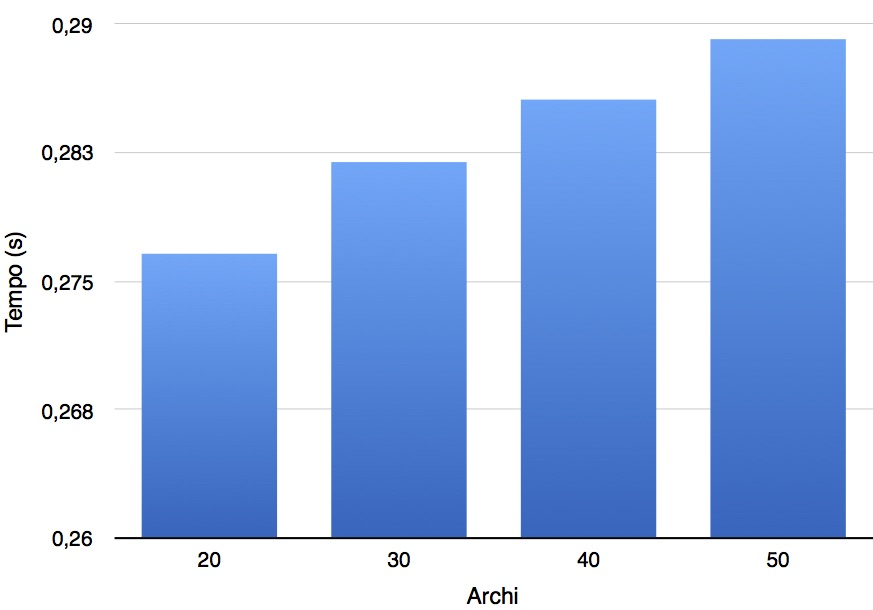
\includegraphics[scale=.25]{img/beta4/10_4.jpg}
		\caption{Algoritmo Partition2}
	\end{minipage}\hfill
	% <-- needed to keep the imgs side by side
	\begin{minipage}{0.40\textwidth}
		\centering
		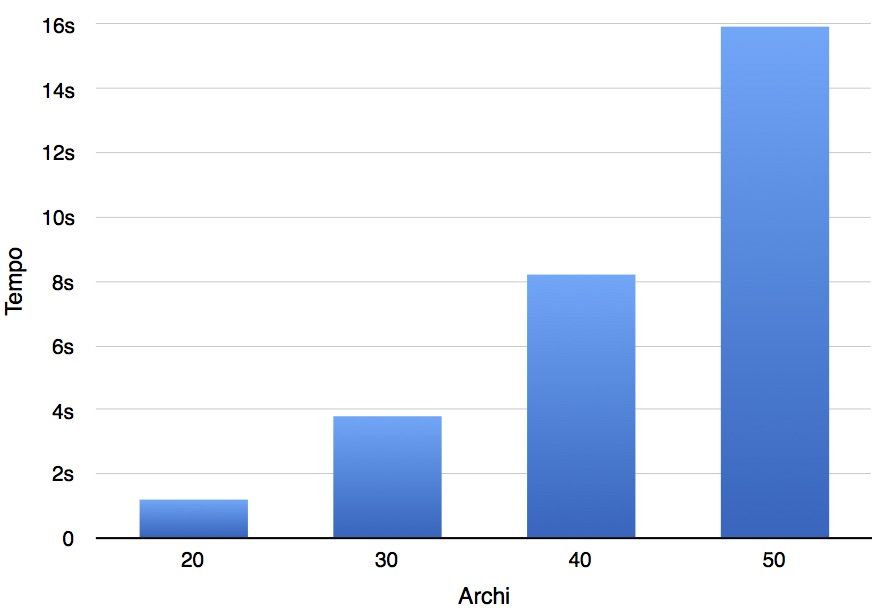
\includegraphics[scale=.25]{img/iole_beta4/iole_10_4.jpg}
		\caption{Algoritmo Partition}
	\end{minipage}
	\caption*{\textit{n = 10}}
\end{figure}
\begin{figure}[h!]
	\vspace*{1cm}
	\begin{minipage}{0.40\textwidth}
		\centering
		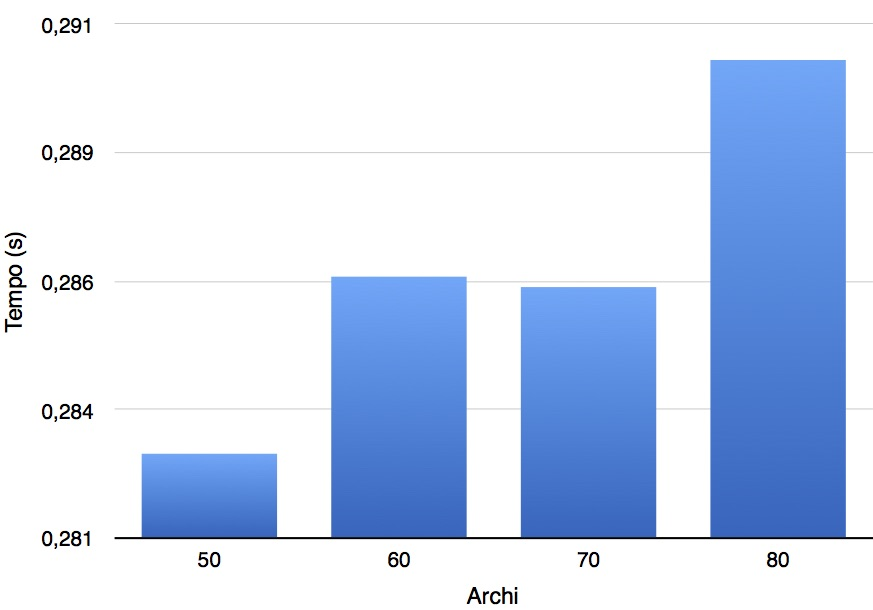
\includegraphics[scale=.25]{img/beta4/15_4.jpg}
		\caption{Algoritmo Partition2}
	\end{minipage}\hfill
	% <-- needed to keep the imgs side by side
	\begin{minipage}{0.40\textwidth}
		\centering
		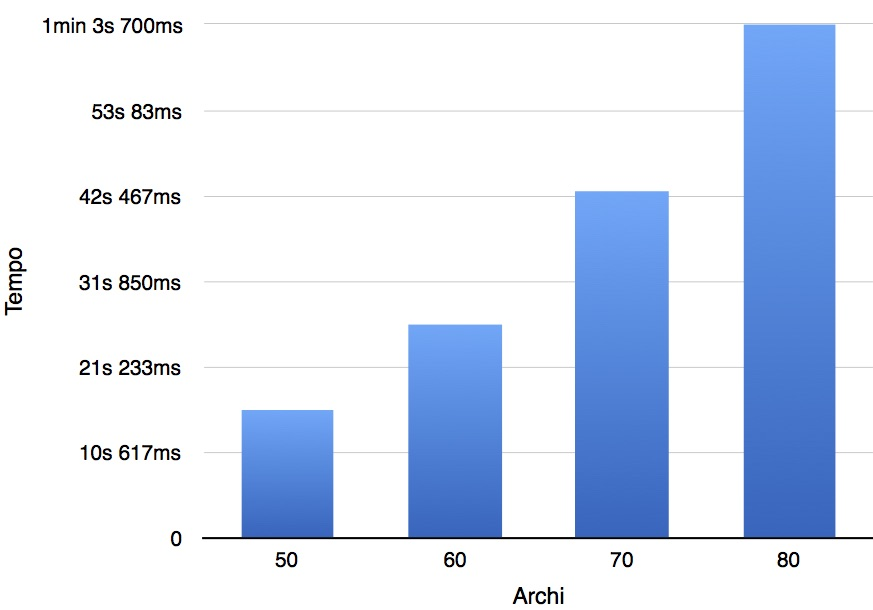
\includegraphics[scale=.25]{img/iole_beta4/iole_15_4.jpg}
		\caption{Algoritmo Partition}
	\end{minipage}
	\caption*{\textit{n = 15}}
\end{figure}
\begin{figure}[h!]
	\vspace*{1cm}
	\begin{minipage}{0.40\textwidth}
		\centering
		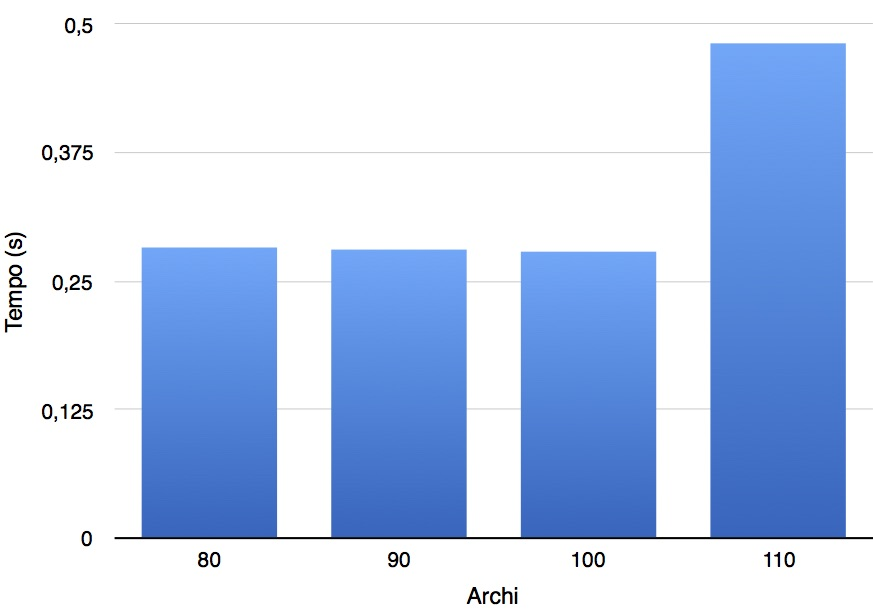
\includegraphics[scale=.25]{img/beta4/20_4.jpg}
		\caption{Algoritmo Partition2}
	\end{minipage}\hfill
	% <-- needed to keep the imgs side by side
	\begin{minipage}{0.40\textwidth}
		\centering
		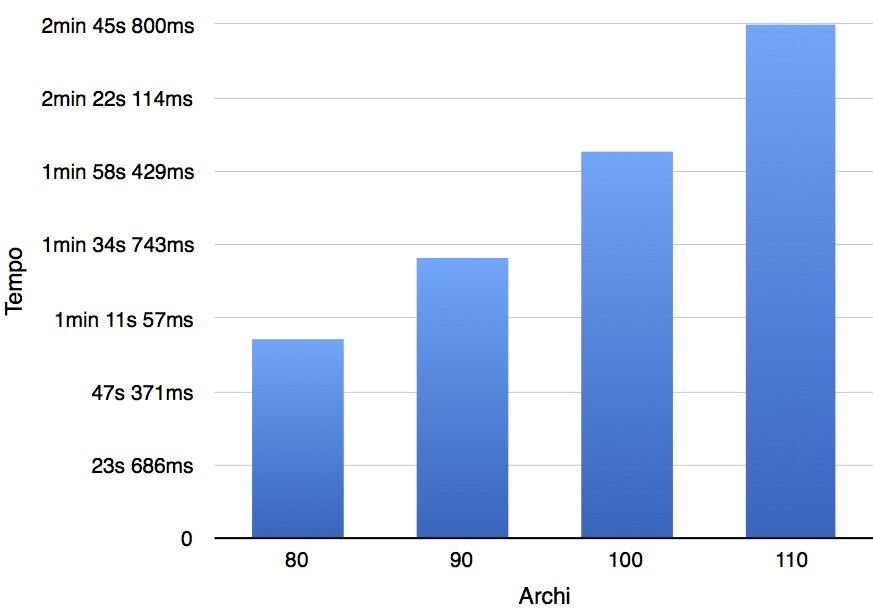
\includegraphics[scale=.25]{img/iole_beta4/iole_20_4.jpg}
		\caption{Algoritmo Partition}
	\end{minipage}
	\caption*{\textit{n = 20}}
\end{figure}
\begin{figure}[h!]
	\vspace*{1cm}
	\begin{minipage}{0.40\textwidth}
		\centering
		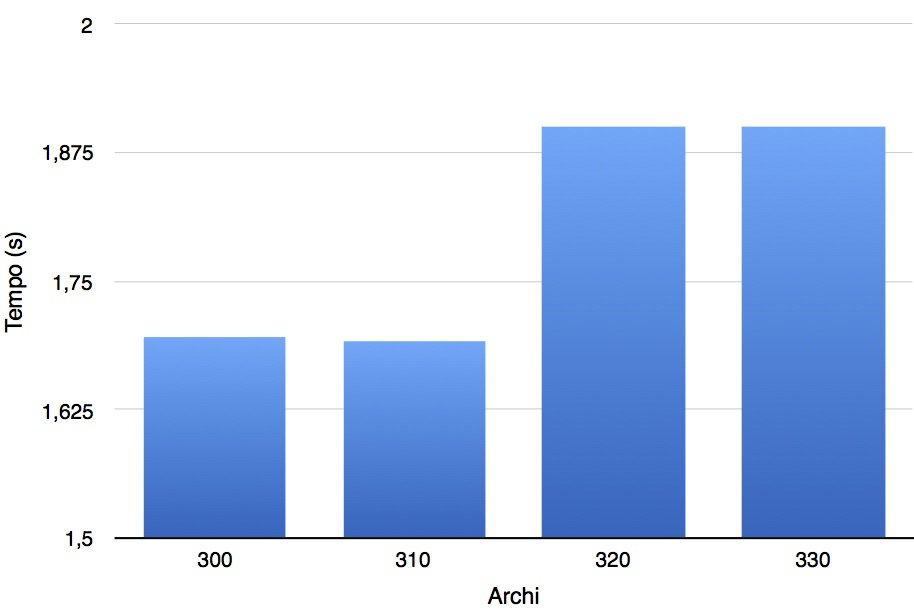
\includegraphics[scale=.25]{img/beta4/35_4.jpg}
		\caption{Algoritmo Partition2}
	\end{minipage}\hfill
	% <-- needed to keep the imgs side by side
	\begin{minipage}{0.40\textwidth}
		\centering
		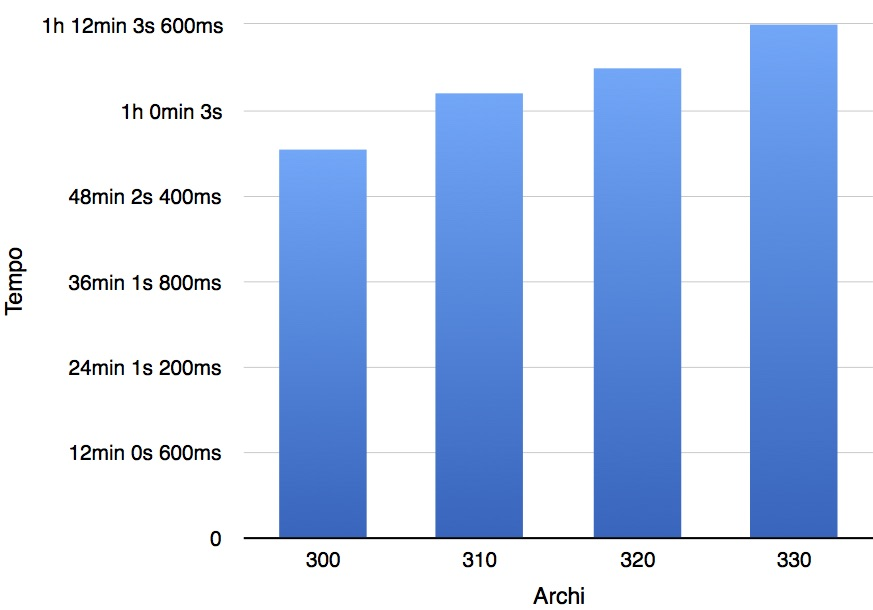
\includegraphics[scale=.25]{img/iole_beta4/iole_35_4.jpg}
		\caption{Algoritmo Partition}
	\end{minipage}
	\caption*{\textit{n = 35}}
\end{figure}
\begin{figure}[h!]
	\vspace*{1cm}
	\begin{minipage}{0.40\textwidth}
		\centering
		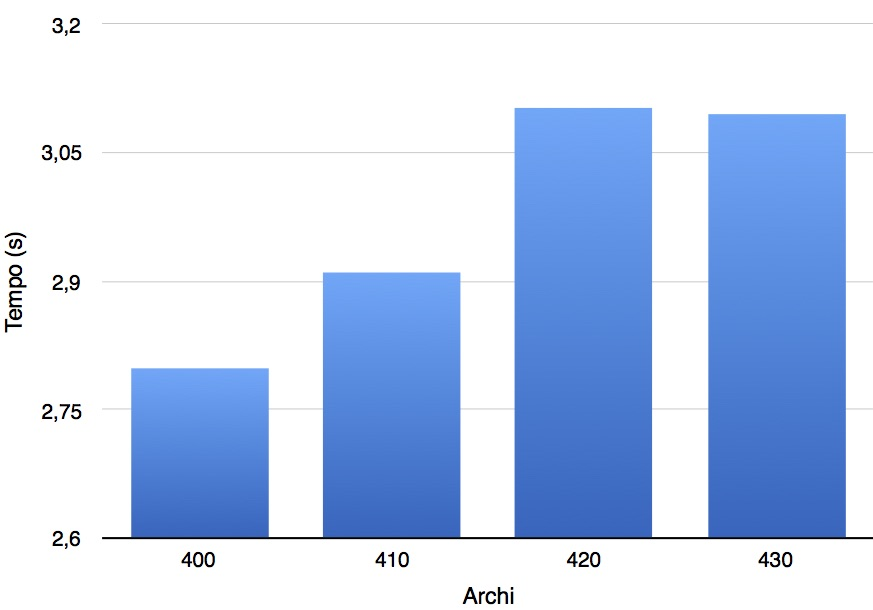
\includegraphics[scale=.25]{img/beta4/40_4.jpg}
		\caption{Algoritmo Partition2}
	\end{minipage}\hfill
	% <-- needed to keep the imgs side by side
	\begin{minipage}{0.40\textwidth}
		\centering
		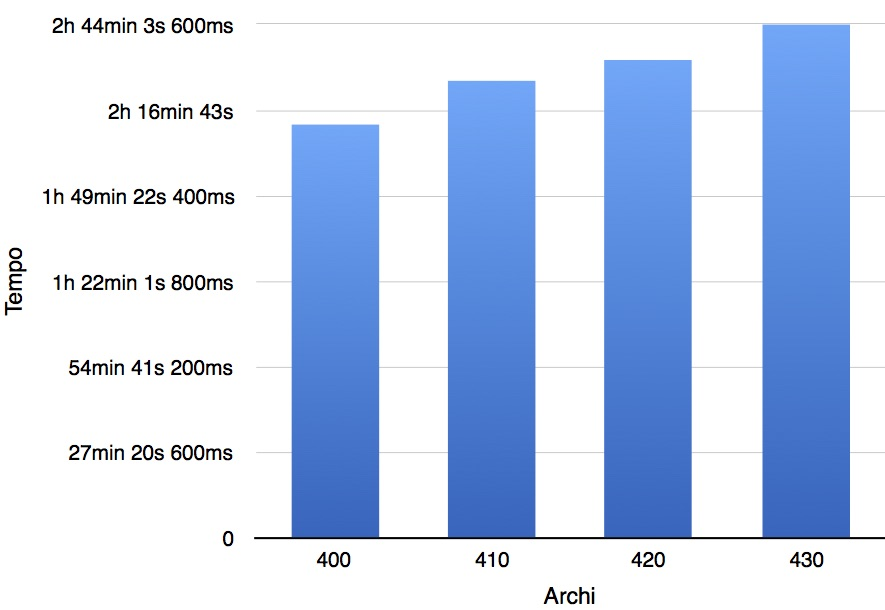
\includegraphics[scale=.25]{img/iole_beta4/iole_40_4.jpg}
		\caption{Algoritmo Partition}
	\end{minipage}
	\caption*{\textit{n = 40}}
\end{figure}
\begin{figure}[h!]
	\vspace*{1cm}
	\begin{minipage}{0.40\textwidth}
		\centering
		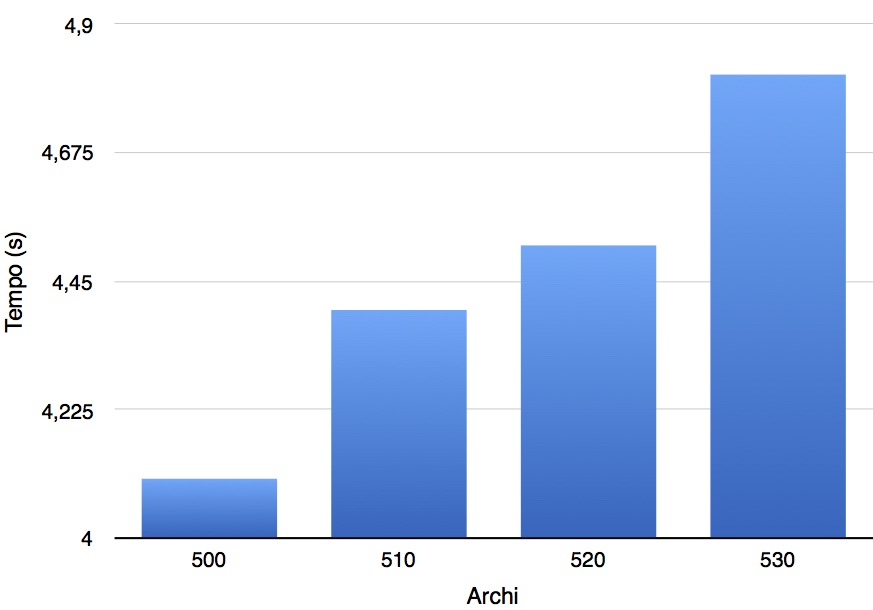
\includegraphics[scale=.25]{img/beta4/45_4.jpg}
		\caption{Algoritmo Partition2}
	\end{minipage}\hfill
	% <-- needed to keep the imgs side by side
	\begin{minipage}{0.40\textwidth}
		\centering
		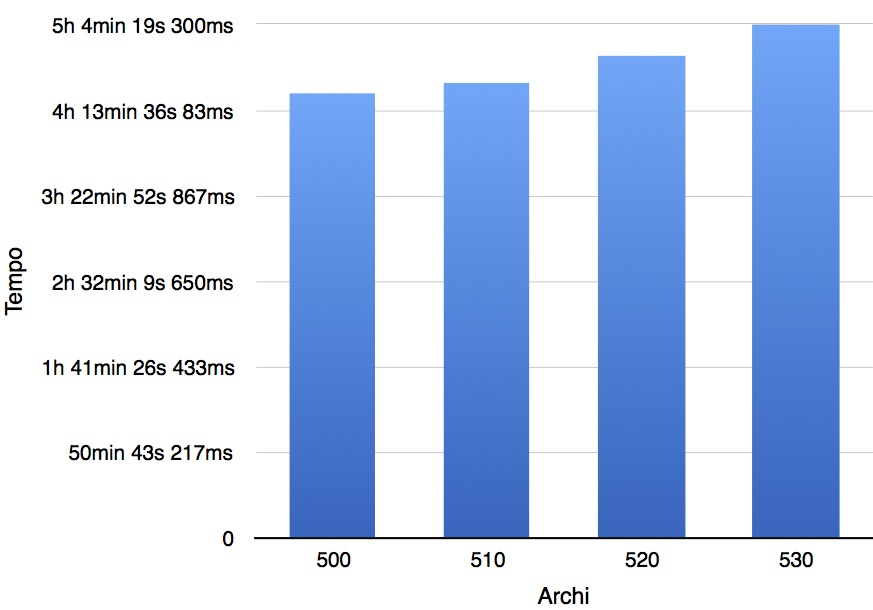
\includegraphics[scale=.25]{img/iole_beta4/iole_45_4.jpg}
		\caption{Algoritmo Partition}
	\end{minipage}
	\caption*{\textit{n = 45}}
\end{figure}
Come è possibile notare dai risultati, l'algoritmo Partition2 ha un netto margine di guadagno in termini di efficienza rispetto all'algoritmo Partition, il quale inizia a soffrire già con un grafo avente 20 nodi ed 90 archi, superando il minuto d'esecuzione contro i 250 ms della versione proposta da questo lavoro di tesi. Di seguito viene mostrato l'andamento del running time per l'algoritmo Partition2 al variare della taglia del grafo nel numero di nodi ed archi. 
\begin{figure}[h!]
	\vspace*{1cm}
	\centering
	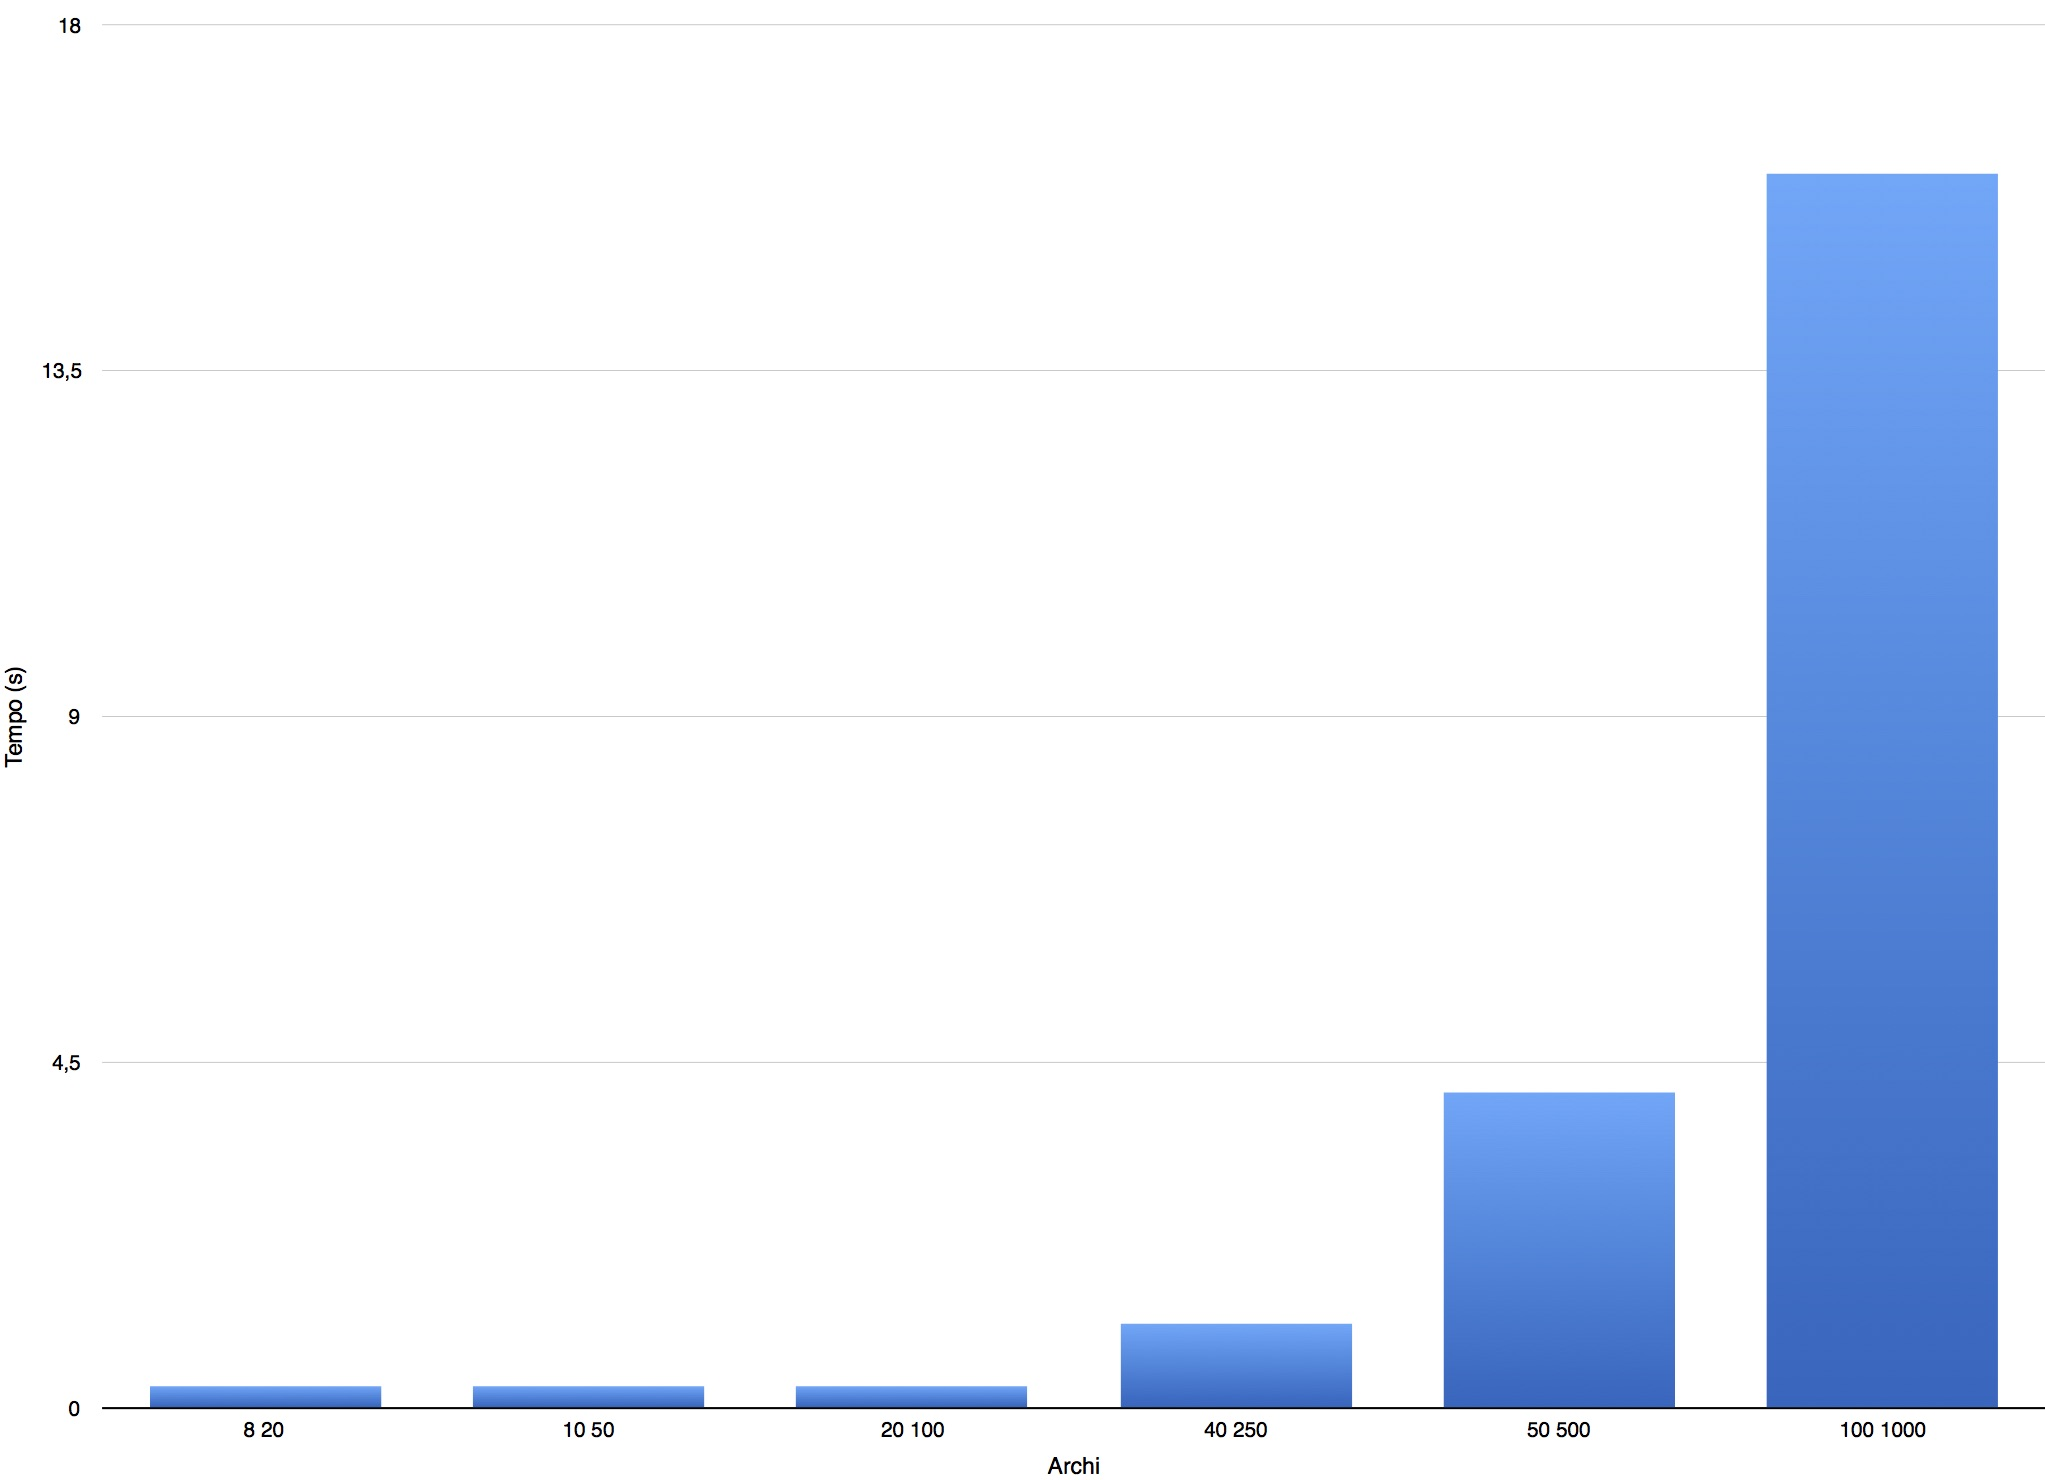
\includegraphics[scale=.15]{img/scala.jpg}
	\caption{Algoritmo Partition2 al variare di n ed m.}
\end{figure}
\begin{table}[]
	\centering
	\begin{tabular}{|c|c|c|c|c|c|c|c|}
		\hline
		n & m & B & $\beta$ & $\epsilon$ & s & t & Tempo (s)\\ \hline
		500 & 1000 & 20 & 0.4 & 0.1 & 1 & 2 & 399.465704\\ \hline
	\end{tabular}
	\caption{Algoritmo Partition2 \textit{n = 500, m = 5000}.}\label{tab:5000}
\end{table}
L'esecuzione riportata in Tabella \ref{tab:5000} è stata tenuta fuori dal precedente grafico per motivi di scala: è possibile apprezzare l'efficienza dell'algoritmo Partition2 anche in questo caso, in quanto impiega circa 400 secondi per calcolare la funzione di partizione su un grafo con 500 nodi e 5000 archi, che già si avvicina ad un'istanza del mondo reale.\\
Grazie ai miglioramenti ottenuti, si è scelto di eseguire anche un test su grafi di dimensioni maggiori, sempre al variare dei parametri $n$ ed $m$, mantenendo i parametri $B = 20, \beta = 0.4, \epsilon = 0.1$ invariati.
\begin{figure}[h!]
	\vspace*{1cm}
	\begin{minipage}{0.40\textwidth}
		\centering
		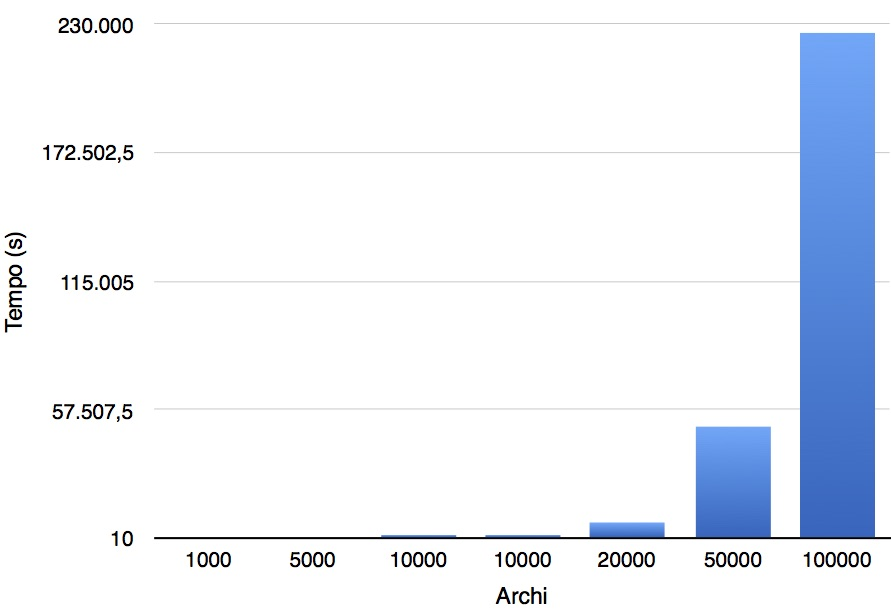
\includegraphics[scale=.25]{img/big.jpg}
		\caption{Scala lineare}
	\end{minipage}\hfill
	% <-- needed to keep the imgs side by side
	\begin{minipage}{0.40\textwidth}
		\centering
		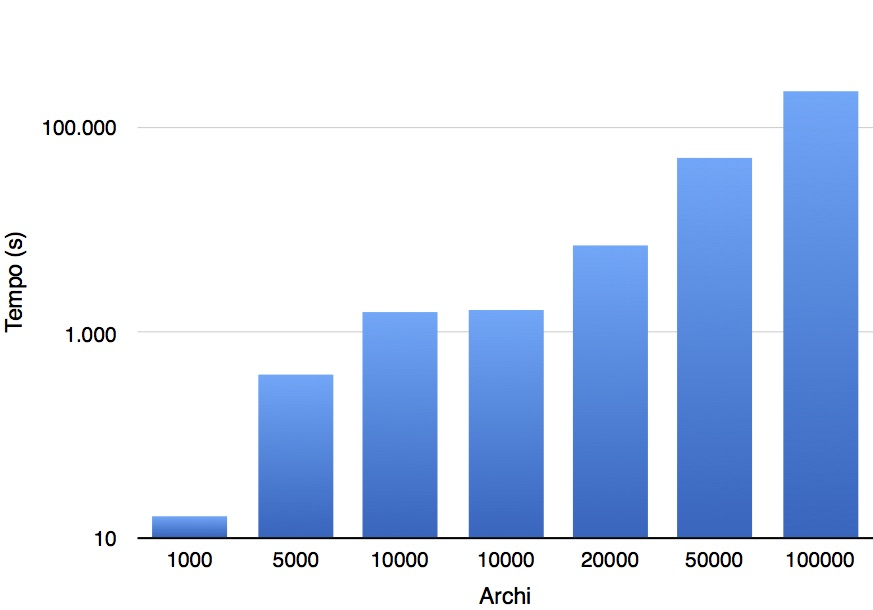
\includegraphics[scale=.25]{img/big_log.jpg}
		\caption{Scala logaritmica}
	\end{minipage}
	\caption*{Grafi di dimensioni maggiori.}
\end{figure}
\clearpage
\subsection{Parametro $\epsilon$}
I seguenti grafici riportano i risultati ottenuti nei test di accuratezza. Il parametro $\epsilon$ è stato fatto variare da $10^{-1}$ a $10^{-4}$.\\
È possibile notare come il tempo aumenti notevolmente nel passaggio da $\epsilon = 10^{-3}$ a $\epsilon = 10^{-4}$, ma sia comunque accettabile anche considerando il fatto che l'algoritmo Partition non è in grado di ottenere tempi ragionevoli già a partire da $\epsilon$ minore di $10^{-1}$.
\begin{figure}[!htb]
	\vspace*{1cm}
	\centering
	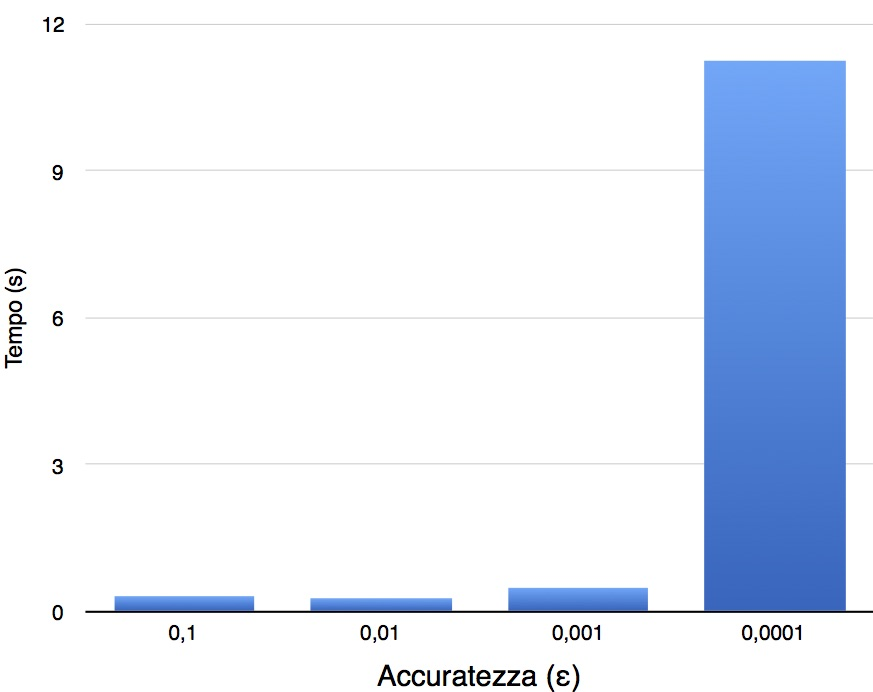
\includegraphics[scale=.3]{img/eps/8.jpg}
	\caption{Algoritmo Partition2 $n = 8, m = 20$.}
\end{figure}
\begin{figure}[!htb]
	\vspace*{1cm}
	\centering
	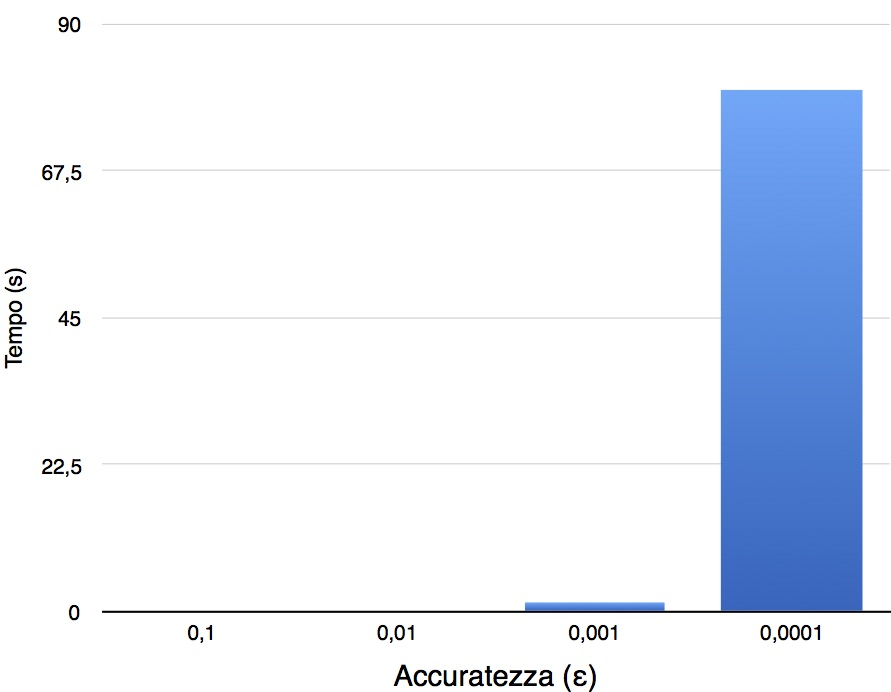
\includegraphics[scale=.3]{img/eps/10.jpg}
	\caption{Algoritmo Partition2 $n = 10, m = 50$.}
\end{figure}
\begin{figure}[!htb]
	\vspace*{1cm}
	\centering
	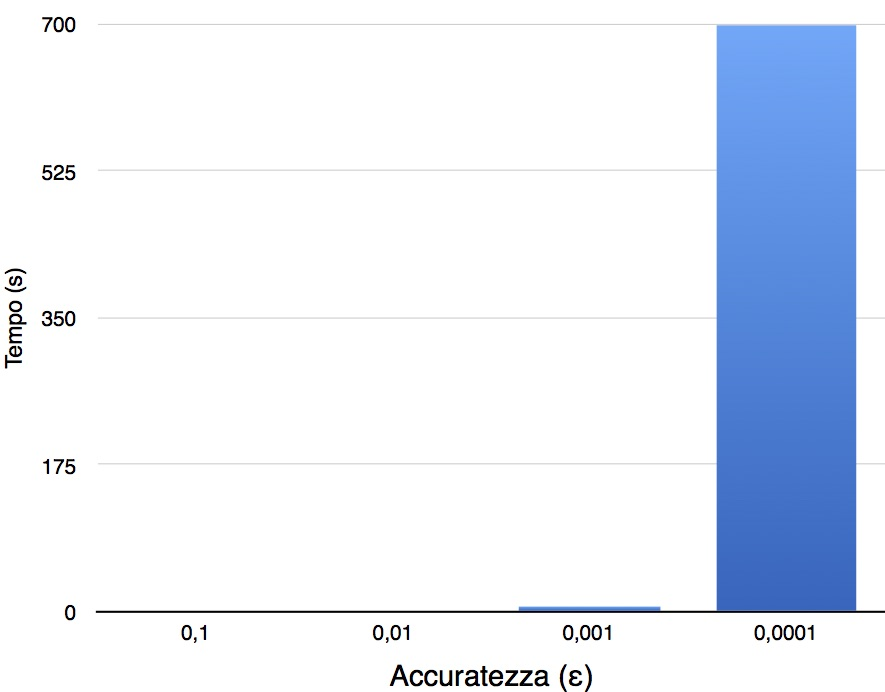
\includegraphics[scale=.3]{img/eps/20.jpg}
	\caption{Algoritmo Partition2 $n = 20, m = 100$.}
\end{figure}
\begin{figure}[!htb]
	\vspace*{1cm}
	\centering
	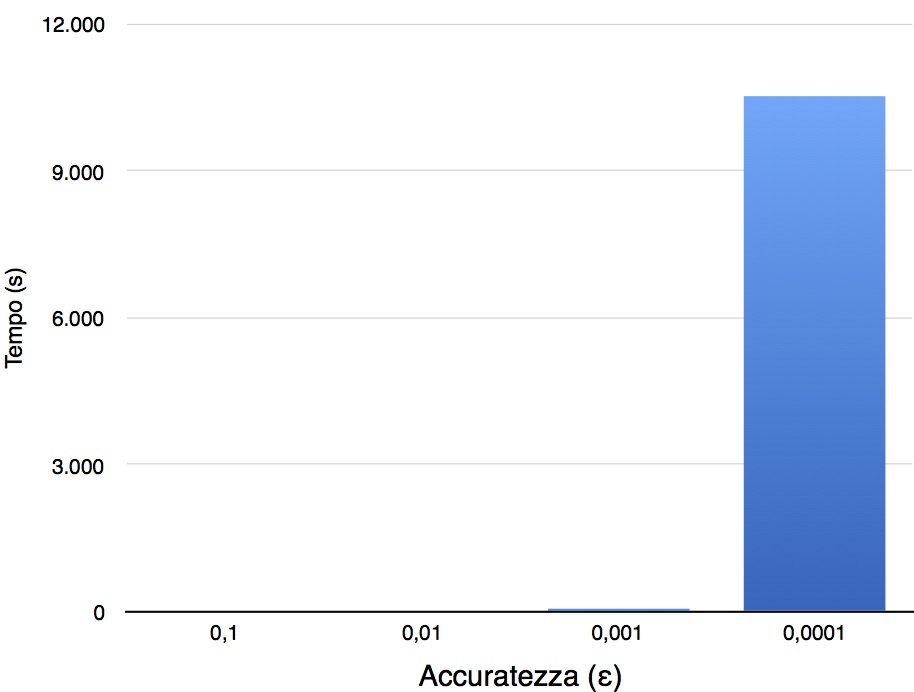
\includegraphics[scale=.3]{img/eps/40.jpg}
	\caption{Algoritmo Partition2 $n = 40, m = 250$.}
\end{figure}
\begin{figure}[!htb]
	\vspace*{1cm}
	\centering
	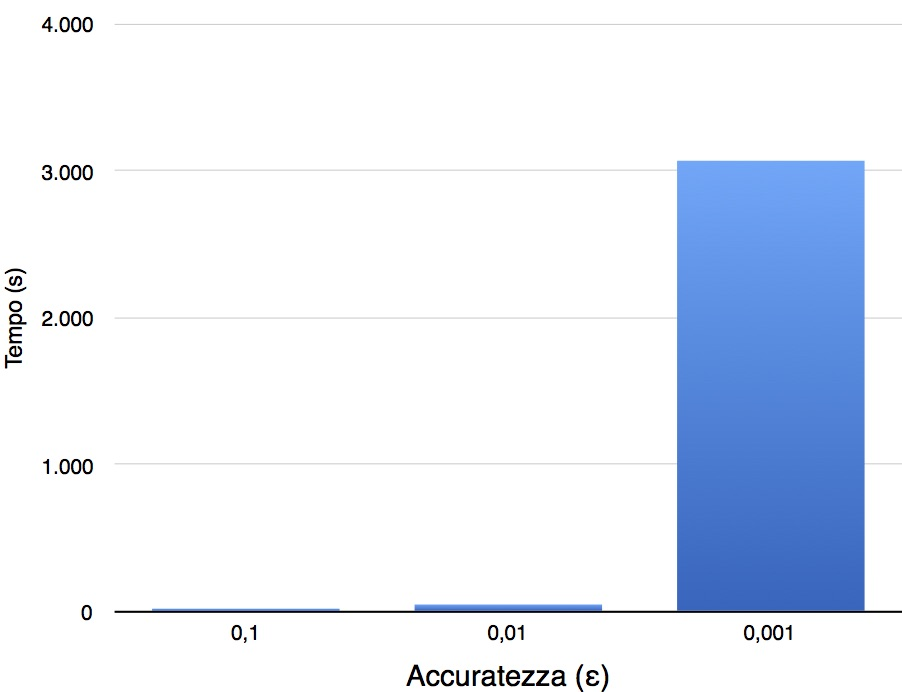
\includegraphics[scale=.3]{img/eps/100.jpg}
	\caption{Algoritmo Partition2 $n = 100, m = 1000$.}
\end{figure}
\clearpage
\subsection{Parametro $\mu$}
I grafici presenti in questa sezione rappresentano l'andamento dell'algoritmo Partition2 al variare dei valori $B$ e $\beta$. Come si ricorda in \ref{mu}, da tali valori dipende $\mu$ e di conseguenza sulla complessità del generatore atto a simulare la catena di Markov, per il Teorema \ref{thm:gen}. Il valore di $B$ è stato fatto variare da 20 ad 8 in tutti i test seguenti, modificando di conseguenza $\beta$ (parametro di razionalità) per mantenere $\mu$ in un range tra 1 e 0.75, come mostrato in Tabella \ref{tab:bbetamu}.
\begin{table}[]
	\centering
	\begin{tabular}{|c|c|c|}
		\hline
		B  & $\beta$  & $\mu$               \\ \hline
		20 & 0.4      & 0.99999977492967584 \\ \hline
		15 & 0.122119 & 0.95000040724956369 \\ \hline
		10 & 0.147222 & 0.90000009697914363 \\ \hline
		12 & 0.104679 & 0.84999866466785234 \\ \hline
		10 & 0.109861 & 0.799999176077972   \\ \hline
		8  & 0.121619 & 0.74999865489104856 \\ \hline
	\end{tabular}
	\caption{Parametri utilizzati.}
	\label{tab:bbetamu}
\end{table}
\begin{figure}[h!]
	\vspace*{1cm}
	\centering
	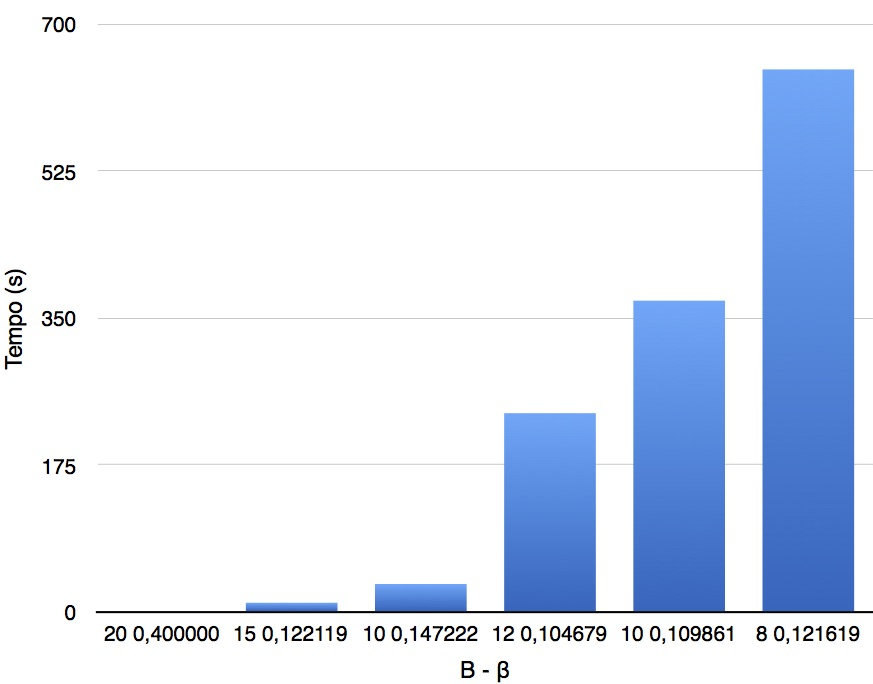
\includegraphics[scale=.3]{img/Bbeta/8_20.jpg}
	\caption{Algoritmo Partition2 $n = 8, m = 20$.}
\end{figure}
\begin{figure}[h!]
	\vspace*{1cm}
	\centering
	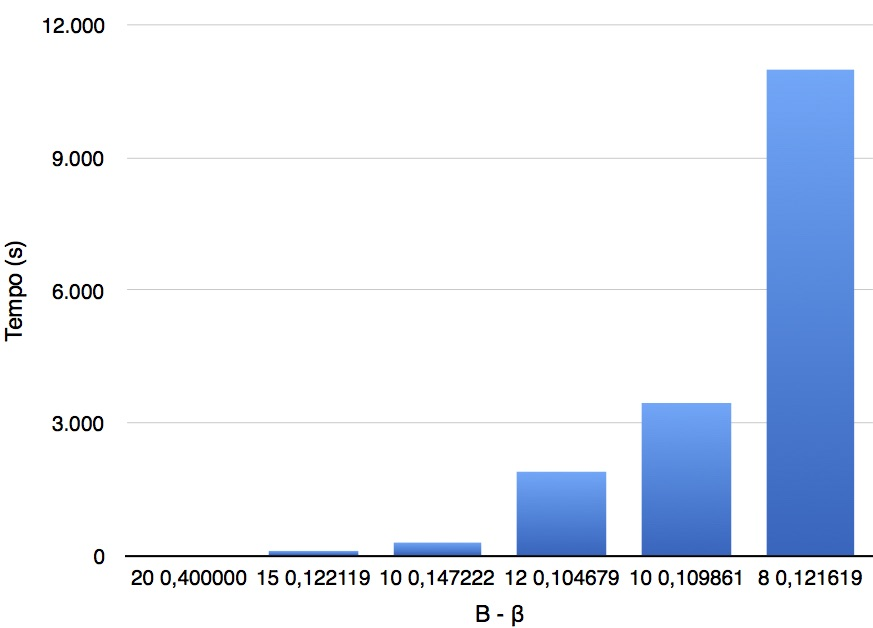
\includegraphics[scale=.3]{img/Bbeta/10_50.jpg}
	\caption{Algoritmo Partition2 $n = 10, m = 50$.}
\end{figure}
\begin{figure}[h!]
	\vspace*{1cm}
	\centering
	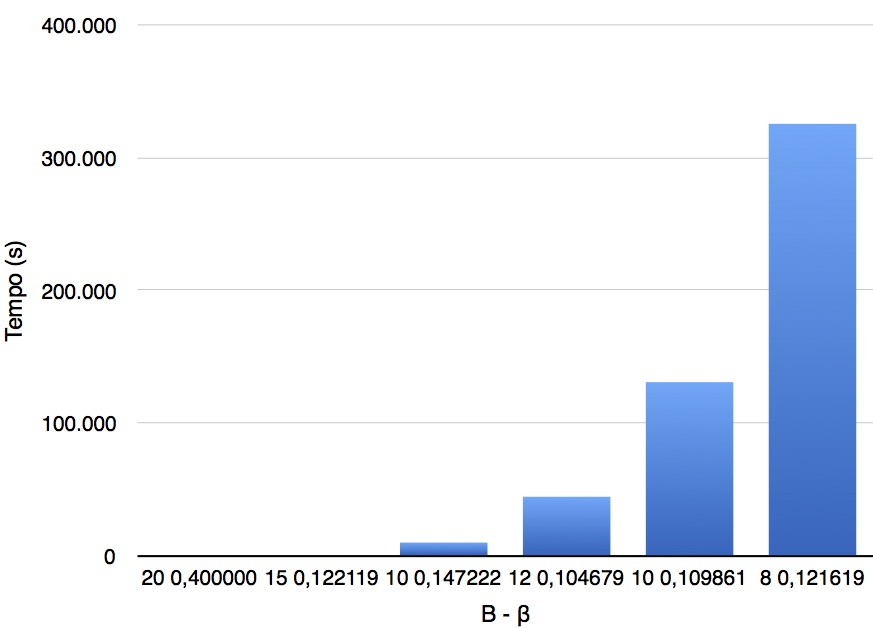
\includegraphics[scale=.3]{img/Bbeta/20_100.jpg}
	\caption{Algoritmo Partition2 $n = 20, m = 100$.}
\end{figure}
\begin{figure}[h!]
	\vspace*{1cm}
	\centering
	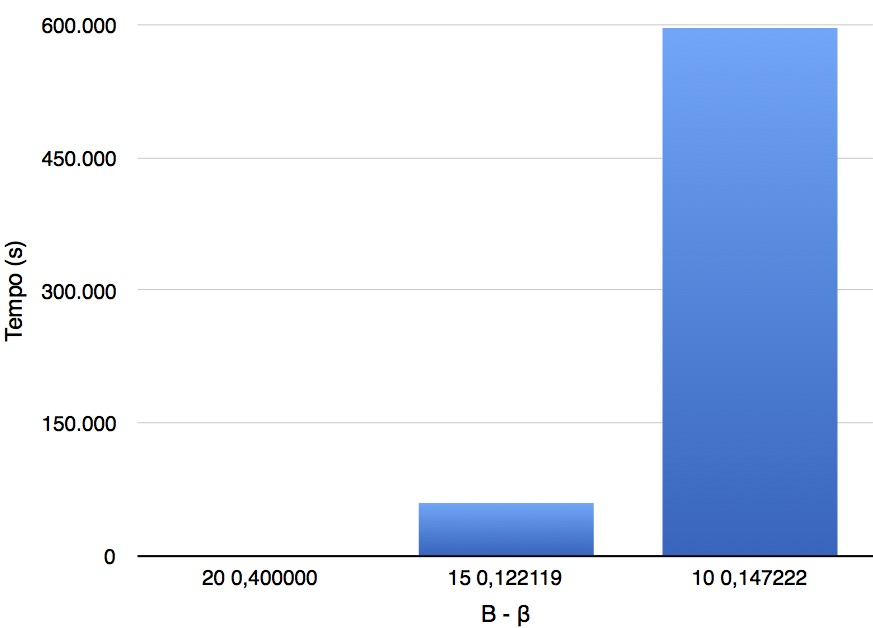
\includegraphics[scale=.3]{img/Bbeta/40_250.jpg}
	\caption{Algoritmo Partition2 $n = 40, m = 250$.}
\end{figure}
È possibile notare dai risultati ottenuti come, al decrescere di $\mu$ il tempo cresca piuttosto linearmente, confermando quanto indicato dal Teorema \ref{thm:gen}.
\clearpage



\section{The Effectiveness of Advertising}
Questa sezione presenta un esempio di applicazione dell'algoritmo sviluppato: la simulazione di una campagna pubblicitaria. si hanno due prodotti da promuovere e si è interessati a calcolare la \textit{magnetizzazione} del sistema, ovvero il numero atteso di persone che sceglieranno di utilizzare un prodotto piuttosto che l'altro. Per raggiungere tale scopo è necessario sfruttare il lavoro proposto nel Capitolo \ref{chap6} riguardante il \textit{mean magnetic moment}.
\subsection{Scenario}
Si consideri una \textit{network} $G = (V,E)$ con $|V| = n$, in cui ogni vertice rappresenta un giocatore (agente) avente a disposizione due possibili scelte, cioè i due prodotti, detti anche \textit{strategie}, denotati da 0 e 1.\\
Ad ogni agente della rete è assegnato un \textit{profilo} $x = (x_1, \cdots, x_n) \in \Omega = {0, 1}^n$. Ad ogni arco $e = (u, v) \in E$ è associato un \textit{two-player game} con funzione potenziale 
\begin{equation}
\Phi_e(x) = 
\begin{cases}
-a, & \text{se}\ x_u = x_v = 1;\\
-b, & \text{se}\ x_u = x_v = 0;\\
0, & \text{altrimenti}
\end{cases}
\label{potentfun}
\end{equation}
con $a, b \geq 0$. Si assume che ogni agente preferisca coordinarsi con i suoi vicini piuttosto che giocare una strategia differente.\\
Si consideri ora la situazione in cui ogni agente debba scegliere una strategia e giocare tale strategia in ogni gioco in cui esso è coinvolto, cioè su ogni arco adiacente. Questa situazione modella un gioco con funzione potenziale
\begin{equation*}
	\Phi(x) = \sum_{e\in E}{\Phi_e(x)}.
	\label{eqpotfun}
\end{equation*}
È noto che la \textit{Logit Dynamics} per questo tipo di gioco converge alla distribuzione
\begin{equation*}
	\pi(x) = \frac{e^{\beta\Phi(x)}}{Z},
	\label{logitdistr}
\end{equation*}
dove Z è il fattore di normalizzazione e $\beta$ rappresenta il livello di razionalità.\\
Tenendo a mente la definizione di \textit{mean magnetic moment} fornita in \ref{mmm}
\begin{equation*}
\mathcal{M} = \beta^{-1}\partial(lnZ)/\partial\beta,
\end{equation*}
il Teorema \ref{thm:fpras_mmm} che afferma
\textit{ ``Esiste un fpras per il mean magnetic moment $\mathcal{M} = \beta^{-1}\partial(lnZ)/\partial\beta$, dove $Z$ è la partition function di un sistema di Ising ferromagnetico.''}

Sono stati apportati notevoli miglioramenti al metodo di approssimazione della funzione \textit{odd(X)}, come mostrato in \ref{ssec:betteroddx}, che hanno portato alla realizzazione degli algoritmi presentati in \ref{ssec:algooddx}.\\
La simulazione è stata realizzando avvalendosi dell'algoritmo \ref{alg:eoddx}, il quale a sua volta fa uso di \ref{alg:est_f_threshold}. Sono stati scelti i parametri che hanno fornito i migliori risultati nei tempi d'esecuzione degli esperimenti precedenti, cioè $B = 20, \beta = 0.4$ ed $\epsilon = 0.1$.
Il grafico seguente riporta i tempi di alcune esecuzioni, al variare del grafo di input.
\begin{figure}[h!]
	\vspace*{1cm}
	\centering
	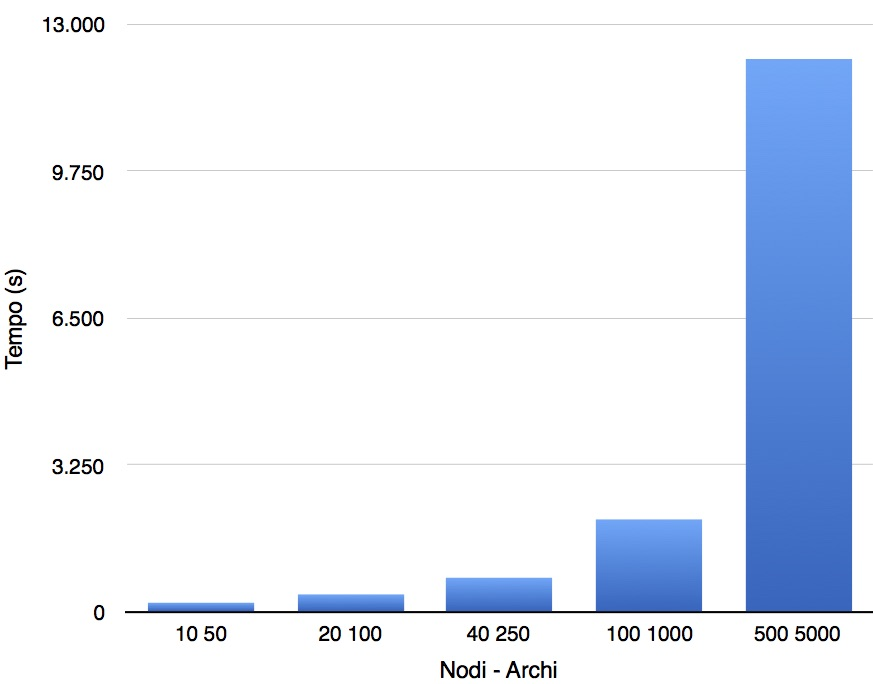
\includegraphics[scale=.3]{img/mmm.jpg}
	\caption{Algoritmo Partition2 $n = 40, m = 250$.}
\end{figure}
La Tabella \ref{tab:mmm} fornisce maggiori informazioni riguardo i dettagli di esecuzione dei test.
\begin{table}[]
	\centering
	\begin{tabular}{|c|c|c|c|c|c|c|c|}
		\hline
		nodi & archi & s & t & Tempo\\ \hline
		10& 50& 5950& 2& 3min 48s\\ \hline
		20& 100& 13218& 2& 6min 31s\\ \hline
		40& 250& 27754& 2& 12min 46s\\ \hline
		100& 1000& 71361& 2& 34min 15s\\ \hline
		500& 5000& 362075& 2& 3h 24min 17s\\ \hline
	\end{tabular}
	\caption{Simulazioni \textit{mean magnetic moment}.}\label{tab:mmm}
\end{table}
Il lavoro \cite{rinaldi2016approximation} riporta nel Capitolo 6 i risultati del test effettuato per un simile scenario e la Tabella \ref{tab:mmmrin} mostra il tempo impiegato per eseguire un test su un grafo con 10 nodi e 50 archi.
\begin{table}[]
	\centering
	\begin{tabular}{|c|c|c|c|c|c|c|c|}
		\hline
		nodi & archi & s & t & Tempo\\ \hline
		10& 50& 62245& 2& 14h 20m 16s\\ \hline
	\end{tabular}
	\caption{Simulazioni \textit{mean magnetic moment}.}\label{tab:mmmrin}
\end{table}
È evidente che tale implementazione sia impraticabile in situazioni reali, e allo stesso tempo è possibile apprezzare l'efficienza del lavoro proposto, che porta a termine lo stesso esperimento in circa 4 minuti rispetto alle 14 ore impiegate in precedenza. Inoltre, l'algoritmo che calcola il \textit{mean magnetic moment} presentato in questa tesi presenta tempi ragionevoli anche su istanza di dimensioni discrete, come nel caso del grafo a 500 nodi e 5000 archi su cui impiega circa 3 ore e 30 minuti per calcolarne la magnetizzazione.
\clearpage
\section{Test su dati reali}
Il lavoro svolto ha reso possibile l'obiettivo preposto: testare l'algoritmo \textbf{Partition2} su dataset provenienti dal mondo reale.\\
\subsection{Dataset Gnutella}
Il dataset utilizzato è una delle network messe a disposizione dallo \textit{Stanford Network Analysis Project} (SNAP) \cite{snapnets} e rappresenta una sequenza di 9 \textit{snapshots} della rete di condivisione file \textit{peer-to-peer} Gnutella a partire da Agosto 2002. I nodi rappresentano gli \textit{host} nella topologia della rete Gnutella e gli archi rappresentano le connessioni tra di essi. In Tabella \ref{tab:gnutella} vengono riportate informazioni dettagliate sul dataset.
\begin{table}[h!]
	\centering
	\begin{tabular}{|c|c|}
		\hline
		Nodi& 6301\\ \hline
		Archi& 20777\\ \hline
		Nodi nella più grande WCC& 6299 (1.000)\\ \hline
		Archi nella più grande WCC& 20776 (1.000)\\ \hline
		Nodi nella più grande SCC& 2068 (0.328)\\ \hline
		Archi nella più grande SCC& 9313 (0.448)\\ \hline
		Coefficiente di average clustering& 0.0109\\ \hline
		Numero di triangoli& 2383\\ \hline
		Frazione di triangoli chiusi& 0.006983\\ \hline
		Diametro (\textit{shortest path} più lungo)& 9\\ \hline
	\end{tabular}
	\caption{Statistiche del grafo Gnutella (SNAP).}\label{tab:gnutella}
\end{table}

L'algoritmo \textbf{Partition2} ha terminato la sua esecuzione in 59.129,02 secondi, cioè in circa 16 ore e 42 minuti.
\subsection{Dataset Facebook}
Il dataset utilizzato in quest'ultimo esperimento è anch'esso messo a disposizione dallo \textit{Stanford Network Analysis Project} (SNAP) \cite{snapnets} e rappresenta uno \textit{snapshot} di un sottografo della rete di amicizie di Facebook. Gli utenti sono rappresentati dai nodi e le relazioni di amicizia sono rappresentate dagli archi. Il grafo in questione è una vera e propria rete sociale e presenta tutte le caratteristiche tipiche di questo tipo di reti, come l'alto numero di triangoli ed un discreto coefficiente di \textit{average clustering}. La Tabella \ref{tab:facebook} mostra ulteriori informazioni sul dataset.\\
\begin{table}[h!]
	\centering
	\begin{tabular}{|c|c|}
		\hline
		Nodi& 4039\\ \hline
		Archi& 88234\\ \hline
		Nodi nella più grande WCC& 4039 (1.000)\\ \hline
		Archi nella più grande WCC& 88234 (1.000)\\ \hline
		Nodi nella più grande SCC& 4039 (1.000)\\ \hline
		Archi nella più grande SCC& 88234 (1.000)\\ \hline
		Coefficiente di average clustering& 0.6055\\ \hline
		Numero di triangoli& 1612010\\ \hline
		Frazione di triangoli chiusi& 0.2647\\ \hline
		Diametro (\textit{shortest path} più lungo)& 8\\ \hline
	\end{tabular}
	\caption{Statistiche del grafo Facebook (SNAP).}\label{tab:facebook}
\end{table}
L'algoritmo \textbf{Partition2} ha terminato la sua esecuzione in 684.060,44 secondi, cioè circa 7 giorni. Considerando le caratteristiche della rete, il tempo impiegato non è eccessivo.\\
Questo prova l'effettiva possibilità di poter essere utilizzato su reti del mondo reale.
\clearpage

%%%%%%%%%%%%%%%%%%%%%%%%%%%%
\chapter{Conclusioni e sviluppi futuri}
In questo lavoro di tesi è stata proposta una versione migliorata dell'algoritmo per il calcolo della \textit{partition function} Z di un sistema di Ising ferromagnetico arbitrario in \ref{chap5}, che fosse superiore nelle prestazioni rispetto a quello presentato nel lavoro \cite{rinaldi2016approximation}.\\
I risultati ottenuti durante la fase di testing, analizzati nella sezione \ref{sec:testing}, in particolare dal confronto con la versione sviluppata in \cite{rinaldi2016approximation}, rendono possibile verificare il netto miglioramento ottenuto nel \textit{running time} dell'algoritmo.\\
Tali risultati sono stati il frutto di una attenta analisi dei Teoremi, Lemmi ed assunzioni (a volte approssimative) del lavoro di Jerrum e Sinclair \cite{jerrum1993polynomial}, spesso seguita da una rivisitazione che puntasse alla correttezza ma soprattutto all'efficienza.\\
Le performance raggiunte consentono, ora, di utilizzare il lavoro sviluppato per calcolare la funzione di partizione Z in una particolare dinamica, e quindi di computare la probabilità stazionaria in tempo un \textit{polinomiale} trattabile in casi concreti, caratteristica che fino ad ora non era possibile ottenere con gli algoritmi precedenti, i quali sebbene avessero complessità polinomiale non consentivano di trattare casi reali, a causa del \textit{running time} molto sensibile anche ad un piccolo incremento nella taglia dell'input.\\
L'efficienza dell'algoritmo proposto deriva dal lavoro svolto nell'ottimizzazione dei valori \textit{s} e \textit{t} che rappresentano, rispettivamente, la taglia dell'insieme di configurazioni su cui eseguire il generatore del Teorema \ref{thm:gen} ed il numero di ripetizioni dell'esperimento necessarie su cui calcolare la mediana. Il generatore del \textit{subgraphs-world process}, descritto in \ref{sec:pf}, è stato migliorato notevolmente sia dal punto di vista dell'ottimizzazione del codice, come del resto tutto il codice implementato, ma soprattutto nella sua complessità computazionale: il precedente tempo d'esecuzione era limitato da $O(m^2\mu^{-8}(log\,\delta^{-1} + m))$, pertanto era fortemente influenzato dal numero di archi del grafo di input; grazie all'integrazione del lavoro \cite{auletta2011convergence}, come mostrato in \ref{sec:mypf}, la complessità è stata portata a $O(2m^2\mu^{-4}(log\,\delta^{-1} + 1))$, riducendo così di molto la dipendenza dal numero di archi.\\
Gli sviluppi futuri più interessanti riguardano il generatore. La direzione da prendere sarebbe quella di lavorare sulla catena di Markov da simulare ed in particolare un importante passo avanti prevederebbe la sua parallelizzazione, operando sulla matrice di transizione: tale miglioramento porterebbe un notevole incremento prestazionale, consentendo di effettuare esperimenti anche su reti sociali di elevata dimensione, così da poterne computare la magnetizzazione e ad esempio poter contribuire concretamente nel campo del \textit{computational advertising}.


\begin{thebibliography}{}
\addcontentsline{toc}{chapter}{Bibliografia}% inserisce nell'indice la bibliografia

\bibitem{1}{W.Shen, D.H. Norrie, Agent-Based Systems for Intelligent
Manufacturing: A State-of-the-Art Survey, Knowledge and Information
Systems, an Int. Jour. 1, 2, (1999) 129-156.}

\bibitem{2}{Boids \url{http://en.wikipedia.org/wiki/Boids}}

\bibitem{3}{Swarm \url{www.santafe.edu/media/workingpapers/96-06-042.pdf}}

\bibitem{4}{MASON \url{http://cs.gmu.edu/~eclab/projects/mason/}}

\bibitem{5}{NetLogo Models Library \url{http://ccl.northwestern.edu/netlogo/models/}}

\bibitem{6}{Axtell, R. L. \& Epstein, J. M. (1996) Growing Artificial Societies: Social Science from the Bottom Up (Brookings Institution Press/MIT Press, Cambridge, MA)}

\bibitem{7}{M.E. Inchiosa \& M.T. Parker, (2002) Overcoming design and development challenges in agent-based modeling using ASCAPE \url{http://www.pnas.org/content/99/suppl_3/7304.full.pdf+html}}

\bibitem{8}{M.J. North, N.T. Collier, J. Ozik, E.R. Tatara, C.M. Macal, M. Bragen and P. Sydelko, (2013) Complex adaptive systems modeling with Repast Simphony \url{http://www.casmodeling.com/content/1/1/3}}

\bibitem{9}{Eclipse Development Process \url{https://www.eclipse.org/projects/dev_process/}}

\bibitem{10}{Eclipse Modeling Framework \url{http://www.eclipse.org/modeling/emf/}}

\bibitem{11}{D. Steinberg, F. Budinsky, M. Paternostro, E. Merks, EMF: Eclipse Modeling Framework 2nd Edition, Addison-Wesley Professional}

\bibitem{12}{M.Amoruso, (2013) Progettazione assistita di simulazioni agent-based: l'integrazione di una nuova target platform in Agent Modeling Platform}

\end{thebibliography}

\end{document}
